\chapter{Recherche de nouvelle physique dans les \'ev\'enements \`a quatre quarks top}
\label{chap:Recherche4tops}

La recherche d'\'ev\'enements avec quatre quarks top dans l'\'etat final ainsi que les contraintes pos\'ees sur quelques mod\`eles pr\'edisant ce type d'\'ev\'enements sont pr\'esent\'ees dans ce chapitre. 
Tout ce qui s'y trouve est, comme pour les travaux pr\'esent\'es pr\'ec\'edemment,  le fruit d'un travail collectif. Le nombre de personnes impliqu\'ees est trop grand pour pouvoir toutes les citer ici. Les principales personnes avec qui j'ai travaill\'e sont David Calvet, Daniela Paredes, Lo\"ic Val\'ery et Dorian Simon.  

Les motivations pour r\'ealiser une telle recherche sont pr\'esent\'ees dans la section~\ref{sec:introFourTops}. 
Les mod\`eles contraints sont pr\'esent\'es dans la section~\ref{sec:models}. Enfin, l'analyse et les limites d'exclusion obtenues sont pr\'esent\'ees dans la section~\ref{sec:analyseFourTops}. 
Mon activit\'e ayant port\'e principalement sur des \'etudes pr\'eliminaires de sensibilit\'e, le choix des mod\`eles et l'interpr\'etation statistique des donn\'ees, l'analyse en elle-m\^eme ne sera que tr\`es bri\`evement d\'ecrite. 
Pour plus de d\'etails, le lecteur est invit\'e \`a consulter les manuscripts de th\`ese des \'etudiants ayant travaill\'es sur ce sujet~\cite{paredeshernandez:tel-00921146,valery:tel-01079982,doriansimonPhD}, les notes de conf\'erences~\cite{ATLAS-CONF-2012-130,ATLAS-CONF-2013-051} et l'article~\cite{Aad:2015gdg}. 

\section{Introduction}
\label{sec:introFourTops}

Bien que jamais mis en d\'efaut exp\'erimentalement, le mod\`ele standard de la 
physique des particules 
est consid\'er\'e comme \'etant un mod\`ele effectif cessant d'\^etre valable 
pour des \'energies proches du TeV. 
Un des objectifs principaux des exp\'eriences actuelles, maintenant qu'un 
excellent candidat au boson BEH a \'et\'e d\'ecouvert, 
est la recherche de signes de nouvelle physique \`a cette \'echelle 
d'\'energie. 
Des arguments de nature th\'eorique laissent penser que, s'il y a de la nouvelle 
physique, elle devrait se manifester dans le secteur du quark 
top~\cite{Peskin:2015kka}. 
%Beaucoup des mod\`eles propos\'es pour d\'ecrire cette nouvelle physique pr\'edisent l'existence de nouvelles particules se couplant fortement au quark top. 
L'\'etude de la production et de la d\'esint\'egration de ce quark dans les 
collisions 
proton-proton du LHC est par cons\'equent une voie de recherche int\'eressante 
pour la recherche de nouvelle physique. 
%La recherche d'\'etats finaux avec des quarks top dans les collisions 
%proton-proton du LHC est par cons\'equent une voie de recherche int\'eressante 
%pour la recherche de nouvelle physique. 

Le travail pr\'esent\'e dans ce chapitre s'inscrit dans cette voie. Il est n\'e 
du constat qu'il y avait, dans le champ ph\'enom\'enologique, une activit\'e 
qui n'avait jusqu'alors pas re\c cu l'attention de la communaut\'e 
exp\'erimentale et qui pourtant semblait prometteuse. Cette activit\'e portait 
sur l'\'etude de mod\`eles dans lesquels le quark top est composite 
\cite{PhysRevD.51.3888,PhysRevD.78.074026,1126-6708-2008-04-087,
1126-6708-2009-05-022}, 
de mod\`eles de dimensions suppl\'ementaires \cite{Guchait:2007jd}
ou encore des mod\`eles dans lesquels des scalaires color\'es sont produit par paire au LHC \cite{Chen:2008hh,Gerbush:2007fe}.
% ou encore de mod\`eles dans lesquels le top se couple fortement au secteur responsable de la brisure de la sym\'etrie \'electrofaible \cite{Cheung:1995eq,Spira:1997ce}. 
Une des pr\'edictions de ces mod\`eles est la production accrue d'\'ev\'enements avec quatre quarks top (\fourtop) dans l'\'etat final. Cette production est possible dans le mod\`ele standard, cependant sa section efficace est tr\`es faible (environ $1$~fb \`a 8~TeV~\cite{Barger:2010uw}). L'observation d'\'ev\'enements \fourtop{} serait donc une signature claire de la pr\'esence de nouvelle physique. 

Une \'etude pr\'eliminaire de l'\'etat final \fourtop{} se basant sur le mod\`ele pr\'esent\'e dans \cite{1126-6708-2008-04-087} a alors \'et\'e faite. Elle a permis de montrer que le LHC avec les exp\'eriences ATLAS et CMS \'etait capable de contraindre fortement les mod\`eles pr\'edisant cet \'etat final. Ceci nous a conduit \`a mettre en place une strat\'egie d'analyse pour rechercher les \'ev\'enements \fourtop{} avec les donn\'ees recueillies par le d\'etecteur \ATLAS~\`a 7 et 8~TeV. Les mod\`eles recherch\'es sont d\'ecrits dans la section~\ref{sec:models}. Les analyses r\'ealis\'ees ainsi que les contraintes mises sur ces mod\`eles sont d\'ecrites dans la section~\ref{sec:analyseFourTops}.

\section{Mod\`eles recherch\'es}
\label{sec:models}

Pour la premi\`ere recherche d'\'ev\'enements \fourtop{} avec les donn\`ees \`a 7~TeV, nous avons choisi un mod\`ele effectif dans lequel les \'ev\'enements \fourtop{} proviennent d'une interaction de contact. Ce mod\`ele non-r\'esonant est, de tous ceux d\'ecrits dans les articles cit\'es ci-dessus, celui qui permet l'\'etablissement de contraintes le plus simplement et de la mani\`ere la plus mod\`ele ind\'ependante possible. Ce mod\`ele est d\'ecrit dans la section~\ref{sec:interactionContact}. 

Suite \`a l'analyse des donn\'ees \`a 7~TeV, nous avons poursuivi avec l'analyse des donn\'ees \`a 8~TeV et \'etendu l'interpr\'etation \`a d'autres modes de production d'\'ev\'enements \fourtop. En effet, durant les ann\'ees 2010, 2011 et 2012 l'activit\'e ph\'enom\'enologique sur des mod\`eles conduisants \`a ce mode de production s'est poursuivie et de nouveau mod\`eles ont vu le jour \cite{Lyon11,Jung:2010ms,Kane:2011zd,Frigerio:2011zg}. Nous avons choisi le mod\`ele nommé 2UED/RPP \cite{Lyon11} (aussi d\'ecrit dans \cite{Lyon09,Lyon12,Lyon4t}) car la physique sous-jacente est très différente de celle conduisant à l'interaction de contact et les événements pr\'esentent une topologie relativement extr\^eme, avec des objets tr\`es \'energ\'etiques. Ce mod\`ele est d\'ecrit dans la section~\ref{sec:modele2UED/RPP}.

En plus des deux mod\`eles pr\'ec\'edemment cit\'es, un autre mod\`ele a \'et\'e consid\'er\'e dans l'analyse des donn\'ees \`a 8~TeV. Il s'agit d'un mod\`ele supersymm\'etrique pr\'edisant la production par paire d'une particule scalaire color\'ee nomm\'ee \english{sgluon}. Le \english{sgluon} se d\'esint\`egre pr\'ef\'erentiellement en une paire $t\bar{t}$, ce qui conduit \`a l'\'etat final \fourtop. 

Les trois modes de production d'\'ev\'enements \fourtop{} consid\'er\'es permettent une interpr\'etation des donn\'ees vari\'ee et compl\'ementaire. Ils correspondent \`a diff\'erents sc\'enarios de nouvelle physique et conduisent \`a des topologies dans l'\'etat final diff\'erentes. Dans la suite, seuls les deux premiers seront discut\'es car ce sont ceux sur lesquels mon travail a port\'e. Le troisi\`eme mod\`ele ainsi que les contraintes qui ont pu \^etre mises sont d\'ecrits dans~\cite{valery:tel-01079982,Aad:2015gdg}.

\subsection{Interaction de contact}
\label{sec:interactionContact}

Le premier mod\`ele sur lequel nous avons cherch\'e \`a mettre des contraintes est un mod\`ele effectif non-r\'esonant d\'ecrit par le lagrangien suivant :
\begin{equation}
\label{eq:LagrangianContactInteraction}
{\cal L} = {\cal L}_\text{SM}+\frac{C}{\Lambda^2}\left(\bar{t}_R\gamma_\mu t_R\right)\left(\bar{t}_R\gamma^\mu t_R\right)
\end{equation}
o\`u ${\cal L}_\text{SM}$ est le lagrangien du mod\`ele standard, $t_R$ est le quark top de chiralit\'e droite, $\gamma_\mu$ les matrices de Dirac, $C$ une constante sans dimension et $\Lambda$ l'\'echelle en \'energie caract\'eristique de la nouvelle physique. Les \'ev\'enements \fourtop{} proviennent donc, dans ce mod\`ele, d'une interaction de contact entre quatre quarks top de chiralit\'e droite. La figure~\ref{fig:feyn4topsContact} montre quelques diagrammes de Feynman pour ce processus. Seule l'interaction de contact avec des quarks de chiralit\'e droite est consid\'er\'ee car celle avec des quarks de chiralit\'e gauche est d\'ej\`a contrainte par les mesures de pr\'ecision \'electrofaible~\cite{PhysRevD.51.3888}. 

\vspace*{0.7cm}
\begin{figure}[!htb]
\begin{center}
\begin{fmffile}{fgraph-ContactGluFu}
\begin{fmfgraph*}(110,60)
\fmfleftn{i}{2}\fmfrightn{o}{4}
\fmfset{curly_len}{2mm}
\fmflabel{$g$}{i1}
\fmflabel{$g$}{i2}
\fmflabel{$t$}{o1}
\fmflabel{$\overline{t}$}{o2}
\fmflabel{$t$}{o3}
\fmflabel{$\overline{t}$}{o4}
\fmf{gluon}{i1,v1}
\fmf{gluon}{i2,v1}
\fmf{gluon,label=$g$}{v1,v2}
\fmf{fermion}{v2,o1}
\fmf{fermion}{v3,v2}
\fmf{fermion}{o2,v3}
\fmf{fermion}{v3,o3}
\fmf{fermion}{o4,v3}
\fmffixedx{20}{i1,v1}
\fmffixedx{20}{i2,v1}
\fmffixed{(25,0)}{v1,v2}
\fmffixed{(25,10)}{v2,v3}
\fmfblob{.07w}{v3}
\end{fmfgraph*} \hspace*{0.8cm} 
\begin{fmfgraph*}(110,60)
\fmfleftn{i}{2}\fmfrightn{o}{4}
\fmfset{curly_len}{2mm}
\fmflabel{$g$}{i1}
\fmflabel{$g$}{i2}
\fmflabel{$t$}{o1}
\fmflabel{$\overline{t}$}{o2}
\fmflabel{$t$}{o3}
\fmflabel{$\overline{t}$}{o4}
\fmf{gluon}{i1,v1}
\fmf{fermion}{v1,o1}
\fmf{fermion}{v2,v1}
\fmf{gluon}{i2,v2}
\fmf{fermion}{v3,v2}
\fmf{fermion}{o2,v3}
\fmf{fermion}{v3,o3}
\fmf{fermion}{o4,v3}
\fmffixedx{30}{i1,v1}
\fmffixedx{30}{i2,v2}
\fmffixedx{34}{v2,v3}
\fmfblob{.07w}{v3}
\end{fmfgraph*} \hspace*{0.8cm} 
\begin{fmfgraph*}(110,60)
\fmfleftn{i}{2}\fmfrightn{o}{4}
\fmfset{curly_len}{2mm}
\fmflabel{$g$}{i1}
\fmflabel{$g$}{i2}
\fmflabel{$t$}{o1}
\fmflabel{$\overline{t}$}{o2}
\fmflabel{$t$}{o3}
\fmflabel{$\overline{t}$}{o4}
\fmf{gluon}{i1,v1}
\fmf{fermion}{v1,o1}
\fmf{fermion}{v2,v1}
\fmf{fermion}{o2,v2}
\fmf{gluon}{i2,v3}
\fmf{fermion}{o4,v3}
\fmf{fermion}{v3,v2}
\fmf{fermion}{v2,o3}
\fmffixedx{40}{i1,v1}
\fmffixedx{40}{i2,v3}
\fmfblob{.07w}{v2}
\end{fmfgraph*} 
\end{fmffile}
\end{center}
\caption{Quelques diagrammes de Feynman de production de quatre quarks top par interaction de contact. \label{fig:feyn4topsContact}}
\end{figure}

L'int\'er\^et de ce mode de production est double. 
Premi\`erement, il n'existe \`a l'heure actuelle que des contraintes tr\`es faibles sur $C/\Lambda^2$ \cite{1126-6708-2009-05-022}. 
Celles-ci proviennent des mesures de section efficace de production de paire $t\bar{t}$ au Tevatron, processus dans lequel l'interaction \`a quatre quarks top appara\^it dans une boucle. L'effet du terme $C/\Lambda^2$ est donc, dans ce processus, relativement supprim\'e. Les \'ev\'enements \fourtop{} apparaissent ainsi compl\'ementaires aux \'ev\'enements $t\bar{t}$ et sondent une physique qu'il n'\'etait pas possible de sonder auparavant. Deuxi\`emement, le terme d'interaction de contact dans l'\'equation~\ref{eq:LagrangianContactInteraction} est un op\'erateur effectif (non renormalisable) qui n'est pas sp\'ecifique \`a un mod\`ele de nouvelle physique en particulier. Cette analyse n'a par cons\'equent pas pour but d'observer ou exclure un mod\`ele particulier mais un ensemble de mod\`eles dans lesquels la nouvelle physique se manifeste, \`a basse \'energie, par une interaction de contact \`a quatre quarks top. C'est le cas par exemple des mod\`eles de top composite et de dimensions suppl\'ementaires pr\'esent\'es dans \cite{PhysRevD.78.074026, 1126-6708-2008-04-087, 1126-6708-2009-05-022, Guchait:2007jd}, qui, \`a haute masse (typiquement sup\'erieure \`a 2~TeV), tendent vers l'interaction de contact.

Le calcul des sections efficaces de production et la g\'en\'eration des \'ev\'enements ont \'et\'e fait avec \madgraph5. Le mod\`ele de physique utilis\'e a \'et\'e fourni par les auteurs de \cite{Degrande:2010kt}. Dans ce mod\`ele, l'interaction de contact n'est pas implément\'ee directement. Elle est obtenue en introduisant une nouvelle particule vectorielle sans couleur ($\rho$) se couplant au quark top de chiralit\'e droite. Ce mod\`ele a deux param\`etres en plus des param\`etres du mod\`ele standard : la constante de couplage entre le quark top et $\rho$ ($g_\rho$) et la masse de $\rho$ ($M_\rho$). Cette derni\`ere est fix\'ee \`a une valeur tr\`es \'elev\'ee pour \^etre dans le r\'egime d'interaction de contact. Dans ce r\'egime, la production d'\'ev\'enements \fourtop{} ne d\'epend que du rapport des deux param\`etres. Dans l'\'equation~\ref{eq:LagrangianContactInteraction}, ce rapport est \'ecrit en terme des param\`etres de la th\'eorie effective ($C$ et $\Lambda$). Ils sont reli\'es \`a $g_\rho$ et $M_\rho$ par l'\'equation suivante : $C/\Lambda^2 = -g_\rho^2/\left(2M_\rho^2\right)$. Il y a donc un unique param\`etre libre.

Pour la g\'en\'eration des \'ev\'enements, la valeur $C/\Lambda^2=-4\pi\TeV^{-2}$ a \'et\'e utilis\'ee. La section efficace de production calcul\'ee avec cette valeur est 42,2~fb \`a $\sqrt{s}=8~$TeV. Il est important de noter que cette valeur de section efficace n'est pas une pr\'ediction du mod\`ele mais un param\`etre libre (puisqu'elle est proportionnelle \`a $C^2/\Lambda^4$) et que la cin\'ematique des \'ev\'enements ne d\'epend pas des valeurs de $C$ et $\Lambda$ (pourvu que la masse $M_\rho$ soit suffisamment grande pour \^etre dans le r\'egime d'interaction de contact). L'acceptance calcul\'ee avec les valeurs utilis\'ees pour la g\'en\'eration peut par cons\'equent \^etre utilis\'ee pour les autres valeurs des param\`etres. L'analyse d\'ecrite dans la section~\ref{sec:analyseFourTops} permet ainsi de poser une limite sup\'erieure sur la section efficace et donc d'exclure certaines r\'egions du plan $\left(C,\Lambda\right)$. 

Lorsque la masse du nouveau vecteur $M_\rho$ n'est pas suffisamment grande pour \^etre dans le r\'egime d'interaction de contact, la production d'\'ev\'enements \fourtop{} ne peut plus \^etre d\'ecrite par l'\'equation~\ref{eq:LagrangianContactInteraction}. La cin\'ematique des \'ev\'enements est de moins en moins dure lorsque $M_\rho$ diminue. Des \'etudes ont \'et\'e r\'ealis\'ees au niveau partonique afin de quantifier la perte en acceptance qui en d\'ecoule. Nous avons montr\'e que la perte entre le r\'egime d'interaction de contact et le r\'egime \`a basse masse n'est pas \'enorme. Lorsque $M_\rho$ passe de 100~TeV \`a 500~GeV, l'acceptance partonique diminue de 30\%. La limite d'exclusion sur la section efficace \`a 500~GeV est donc environ 30\% plus \'elev\'ee que celles obtenues pour l'interaction de contact dans la section~\ref{sec:analyseFourTops}. Il faut toutefois noter que la section efficace de production augmente lorsque la masse diminue. La sensibilit\'e de l'analyse diminue donc de moins de 30\% et elle peut m\^eme augmenter si l'accroissement de la section efficace est plus rapide que la diminution de l'acceptance. Les analyses r\'ealis\'ees sont donc \'egalement sensibles aux sc\'enarios pour lesquels $M_\rho$ est plus petit que $2$~TeV. 

La section efficace de production d'\'ev\'enements \fourtop{} par le mod\`ele standard est faible (environ $1$~fb \`a $\sqrt{s}=8$ TeV) et l'interf\'erence entre cette production et la production par interaction de contact est petite~\cite{Degrande:2010kt}. L'\'echantillon de signal g\'en\'er\'e ne comprend par cons\'equent que la production par interaction de contact. Les densités de partons utilis\'ees sont MSTW2008LO et les \'echelles de renormalisation et factorisation ont \'et\'e fix\'ees \`a $4m_t$, o\`u $m_t$ est la masse du quark top. 

\subsection{Mod\`ele 2UED/RPP}
\label{sec:modele2UED/RPP}

Le modèle 2UED/RPP est un modèle à deux dimensions supplémentaires universelles compactifiées sur le ``Plan Projectif Réel'' (\english{Real Projective Plane}, ou RPP). Son principal intérêt est de prédire un candidat matière noire dont la stabilit\'e est assur\'ee par les sym\'etries du mod\`ele et n'a pas \`a \^etre rajout\'ee de mani\`ere {\it ad hoc}~\cite{Lyon09}.

Du fait de la compactification, l'impulsion est quantifi\'ee suivant les deux dimensions suppl\'ementaires. Il y a donc des tours de Kaluza-Klein pour chaque particule du modèle standard. Les \'etages sont étiquetés par deux entiers $k$ et $l$. Les deux param\`etres du mod\`ele sont les deux rayons de compactification $R_4$ et $R_5$. Plut\^ot que de les utiliser directement, nous utiliserons la masse caract\'eristique $m_{KK}$ et le rapport des rayons $\xi$ donn\'es par
\[m_{KK} = \frac{1}{R_4}\quad\text{et}\quad\xi = \frac{R_4}{R_5}.\]

Au premier ordre, les masses carr\'ees des particules de l'\'etage $(k,l)$ sont $m^2=\frac{k^2}{R_4^2} + \frac{l^2}{R_5^2}$. Les diff\'erences de masse au sein d'un \'etage $(k,l)$ proviennent des corrections d'ordre sup\'erieur. Elles sont petites par rapport aux masses~\cite{Lyon09}.

Le mod\`ele 2UED/RPP est le seul mod\`ele avec moins de trois dimensions suppl\'ementaires universelles qui permet \`a la fois l'existence de fermions chiraux dans l'\'etage $(0,0)$ et l'absence de point ou ligne fixe. La premi\`ere propri\'et\'e est n\'ecessaire pour permettre de retrouver les particules du mod\`ele standard et la deuxi\`eme pour permettre \`a la sym\'etrie assurant la stabilit\'e du candidat mati\`ere d'\^etre non bris\'ee. Ainsi, le candidat mati\`ere noire, qui est la particule la plus l\'eg\`ere de l'\'etage $(1,0)$ (et $(0,1)$ dans le cas o\`u les rayons sont \'egaux) ne peut pas se d\'esint\'egrer en particule du mod\`ele standard. Les mesures de densit\'e relique contraignent $m_{KK}$ \`a se trouver approximativement entre 600~GeV et 1000~GeV~\cite{Lyon12}.

Les événements à quatre quarks top dans ce modèle proviennent essentiellement de la production et de la d\'esinte\'gration de particules lourdes (quarks ou gluons) de l'\'etage $(1,1)$. Pour des raisons de sym\'etries, ces particules sont produites par paire. Chacune d'elle se d\'esint\`egre suivant une chaîne de désintégration qui aboutit \`a la particule la plus l\'eg\`ere de l'\'etage : le photon lourd $A^{(1,1)}$. Les d\'esint\'egrations possibles sont :
\begin{maliste}
\item D\'esint\'egration directe d'un quark : \\
$q_{R/L}^{(1,1)} \rightarrow q A_\mu^{(1,1)} \rightarrow q t \bar{t}$
\item D\'esint\'egration d'un doublet en un boson $Z$ ou $W$ :\\
$q_L^{(1,1)} \rightarrow q Z^{(1,1)} \rightarrow \{q \ell \bar{\ell}^{(1,1)} / q \ell^{(1,1)} \bar{\ell}\} \rightarrow q \ell \bar{\ell}  A_\mu^{(1,1)} \rightarrow q \ell \bar{\ell} t \bar{t}$\\
$q_L^{(1,1)} \rightarrow q' W^{(1,1)} \rightarrow \{q' \ell^{(1,1)} \bar{\nu_\ell} / q' \ell \bar{\nu_\ell}^{(1,1)}\} \rightarrow q' \ell \bar{\nu_\ell} A_\mu^{(1,1)} \rightarrow q' \ell \bar{\nu_\ell} t \bar{t}$
\item D\'esint\'egration d'un gluon : \\
$g_\mu^{(1,1)} \rightarrow q_{R/L}^{(1,1)} q' \rightarrow \dots$
\end{maliste}

Dans ces expressions, $l$ d\'esigne un lepton (incluant les neutrinos dans le cas de la d\'esint\'egration de $Z^{(1,1)}$) et $\nu_l$ le neutrino correspondant dans le cas du $W^{(1,1)}$. $L$ d\'esigne le fermion de l'\'etage $(1,1)$ associ\'e au fermion de chiralit\'e gauche du mod\`ele standard et $R$ celui associ\'e au fermion de chiralit\'e droite.

Les deux photons lourds $A^{(1,1)}$ produits dans l'\'etat final se d\'esint\`egrent suivant un op\'erateur effectif en une paire de particules du mod\`ele standard. Les rapports d'embranchement de ces d\'esint\'egrations ne sont pas pr\'edictibles dans le cadre du mod\`ele 2UED/RPP et constituent donc des param\`etres libres. Cependant, la d\'esint\'egration suppos\'ee la plus importante est celle en une paire $t\bar{t}$~\cite{Lyon11}. L'\'etat final contient donc quatre quarks top et un nombre relativement important de leptons et de quarks du mod\`ele standard. C'est, avec la plus grande impulsion transverse totale, la différence principale avec l'interaction de contact. La figure~\ref{fig:exampleFeynRPP} montre deux diagrammes de Feynman illustrant la production d'\'ev\'enements \fourtop~dans ce mod\`ele. 

\vspace*{0.5cm}
\begin{figure}[!htb]
  \begin{center}

\begin{fmffile}{fgraph-2UEDRPP}
\unitlength = 0.45mm

\begin{fmfgraph*}(160,90)

%\fmfpen{thick}
\fmfleft{i2,i1}
\fmfright{t1,t2,t3,t4}
\fmftop{i1,p1,p2,a5,a6,a7,t4}
\fmfbottom{i2,p3,a1,a2,a3,a4,t1}
\fmfset{curly_len}{2mm}
\fmf{fermion,tension=1}{i1,v1}
\fmf{fermion,tension=.2}{v8,a5}
\fmf{fermion,tension=.2}{a6,v9}
\fmf{fermion,tension=.2}{v10,a7}
\fmf{fermion,tension=.5}{t3,v11,t4}
\fmf{fermion,tension=.2}{a1,v3}
\fmf{fermion,tension=.2}{v4,a2}
\fmf{fermion,tension=.2}{a3,v5}
\fmf{fermion,tension=.2}{v6,a4}
\fmf{fermion,tension=.5}{t1,v7,t2}

\fmf{gluon,tension=1}{i2,v2}


\fmf{gluon,label=${\scriptstyle g}^{\scriptscriptstyle (1,,1)}\;\;$}{v1,v2}
\fmf{gluon,tension=1.2}{v2,v3}
\put(37,33){${\scriptstyle g}^{\scriptscriptstyle (1,1)}$}

\fmf{boson,label=${\scriptstyle W}^{\scriptscriptstyle +(1,,1)}$}{v8,v9}
\fmf{boson,label=${\scriptstyle Z}^{\scriptscriptstyle (1,,1)}$,l.s=left}{v4,v5}
\fmf{boson,tension=0.6}{v6,v7}
\put(120,20){${\scriptstyle A}^{\scriptscriptstyle (1,1)}$}

\fmf{boson,tension=0.6}{v10,v11}
\put(115,62){${\scriptstyle A}^{\scriptscriptstyle (1,1)}$}

\fmf{fermion,tension=1.2,label=${\scriptstyle u_L}^{\scriptscriptstyle (1,,1)}$}{v1,v8}
\fmf{fermion,label=${\scriptstyle \nu_\tau}^{\scriptscriptstyle (1,,1)}$,l.s=right}{v9,v10}
\fmf{fermion,label=$\;\;{\scriptstyle c_{L}}^{\scriptscriptstyle (1,,1)}$,l.s=left}{v3,v4}
\fmf{fermion,label=$\;\;{\scriptstyle \mu}^{\scriptscriptstyle -(1,,1)}\;\;$,l.s=left}{v5,v6}
\fmfblob{.04w}{v11}
\fmfblob{.04w}{v7}
%\fmfv{decor.shape=circle,decor.filled=full,decor.size=10}{v11}
%\fmfv{decor.shape=circle,decor.filled=full,decor.size=10}{v7}

\fmflabel{$u$}{i1}
\fmflabel{$g$}{i2}
\fmflabel{\textcolor{blue}{$\bar{c}$}}{a1}
\fmflabel{\textcolor{blue}{$c$}}{a2}
\fmflabel{\textcolor{blue}{$\mu^+$}}{a3}
\fmflabel{\textcolor{blue}{$\mu^{-}$}}{a4}
\fmflabel{\textcolor{blue}{$d$}}{a5}
\fmflabel{\textcolor{blue}{$\tau^+$}}{a6}
\fmflabel{\textcolor{blue}{$\nu_\tau$}}{a7}
\fmflabel{\textcolor{red}{$\bar{t}$}}{t1}
\fmflabel{\textcolor{red}{$t$}}{t2}
\fmflabel{\textcolor{red}{$\bar{t}$}}{t3}
\fmflabel{\textcolor{red}{$t$}}{t4}

\end{fmfgraph*}
\hspace*{1cm}
\begin{fmfgraph*}(150,80)

%\fmfpen{thick}

\fmfleft{i2,i1}
\fmfright{u1,t1,t2,t3,t4,u2}
\fmfset{curly_len}{2mm}

\fmf{gluon,tension=2}{i1,v1}
\fmf{gluon,tension=2}{i2,v2}
\fmf{fermion}{u1,a1}
\fmf{fermion,tension=2,label=${\scriptstyle \bar{u}_R^{\scriptscriptstyle (1,,1)}}$}{a1,v2}
\fmf{fermion,label=${\scriptstyle u_R^{\scriptscriptstyle (1,,1)}}$}{v2,v1}
\fmf{fermion,tension=2,label=${\scriptstyle u_R^{\scriptscriptstyle (1,,1)}}$}{v1,a2}
\fmf{fermion}{a2,u2}
\fmf{boson,label=${\scriptstyle A^{\scriptscriptstyle (1,,1)}}$}{a1,b1}
\fmf{boson,label=${\scriptstyle A^{\scriptscriptstyle (1,,1)}}$,l.s=right}{a2,b2}
\fmf{fermion,tension=0.8}{t1,b1}
\fmf{fermion,tension=0.5}{b1,t2}
\fmf{fermion,tension=0.8}{t3,b2}
\fmf{fermion,tension=0.5}{b2,t4}

\fmfblob{.04w}{b1}
\fmfblob{.04w}{b2}
%\fmfv{decor.shape=circle,decor.filled=full,decor.size=10}{b1}
%\fmfv{decor.shape=circle,decor.filled=full,decor.size=10}{b2}

\fmflabel{$g$}{i1}
\fmflabel{$g$}{i2}
\fmflabel{\textcolor{blue}{$\bar{u}$}}{u1}
\fmflabel{\textcolor{blue}{$u$}}{u2}
\fmflabel{\textcolor{red}{$\bar{t}$}}{t1}
\fmflabel{\textcolor{red}{$t$}}{t2}
\fmflabel{\textcolor{red}{$\bar{t}$}}{t3}
\fmflabel{\textcolor{red}{$t$}}{t4}
\end{fmfgraph*}
\end{fmffile}
\vspace*{0.4cm}
\caption{Exemple de production d'\'ev\'enements \fourtop~dans le mod\`ele 2UED/RPP.}\label{fig:exampleFeynRPP}
  \end{center}
\end{figure}

La g\'en\'eration des \'ev\'enements \fourtop~est faite en deux \'etapes. Premi\`erement, les paires quark/quark, quark/gluon et gluon/gluon de l'\'etage $(1,1)$ sont produites par \madgraph5. Ensuite, \bridge~est utilis\'e pour r\'ealiser la cha\^ine de d\'esint\'egration jusqu'aux quatre quarks top. Quatre points de masse sont consid\'er\'es : $m_{KK}=600, 800, 1000$ et $1200$~GeV. Dans tous les cas, le rapport d'embranchement de $A^{(1,1)}$ en $t\bar{t}$ est suppos\'e \'egal \`a 1 et le rapport des deux rayons $\xi$ est fix\'e \`a 1. Les sections efficaces de production et les luminosit\'es g\'en\'er\'ees sont donn\'ees dans la table~\ref{tab:MC2UEDRPP}. 
% La figure~\ref{} montre la section efficace totale ainsi que les sections efficaces pour les diff\'erents \'etats initiaux en fonction de $m_{KK}$.

\begin{table}[!htb]
  \begin{center} 
    \begin{tabular}{|c|c|c|} 
      \hline
      $m_{KK}$ (GeV)   &  section efficace (fb) & luminosit\'e (fb$^{-1}$)\\ \hline
      $600$ &  1~285 & 155.5 \\ \hline
      $800$ &  114 & 1709 \\ \hline 
      $1000$ & 11.7 & 12~800 \\ \hline
      $1200$ & 1.22 & 122~600 \\ \hline
    \end{tabular}
    \caption{Section efficace et luminosit\'e g\'en\'er\'ee pour les diff\'erents points de masse consid\'er\'es dans le mod\`ele 2UED/RPP.}\label{tab:MC2UEDRPP}
  \end{center}
\end{table}

% INCERTITUDE ?

\subsection{Production par le mod\`ele standard}

En plus des mod\`eles pr\'esent\'es ci-dessus, la production d'\'ev\'enements \fourtop~dans le mod\`ele standard a \'egalement \'et\'e consid\'er\'ee. Un exemple de diagramme de Feynman est repr\'esent\'e sur la figure~\ref{fig:exampleFeyn4topsSM}. Ce processus n'a jamais \'et\'e observ\'e et la luminosit\'e int\'egr\'ee accumul\'ee au run 1 ne permet pas d'envisager une observation. Il reste cependant int\'eressant d'inclure ce processus dans l'analyse pour \'evaluer la sensibilit\'e atteignable. Un \'echantillon d'\'ev\'enements \fourtop~a par cons\'equent \'et\'e g\'en\'er\'e. Comme pour les mod\`eles pr\'ec\'edents, c'est \madgraph5~qui a \'et\'e utilis\'e.
\vspace*{0.15cm}
\begin{figure}[!htb]
\begin{center}
\begin{fmffile}{fgraph-4topsSM}
\begin{fmfgraph*}(110,60)
\fmfleftn{i}{2}\fmfrightn{o}{4}
\fmfset{curly_len}{2mm}
\fmflabel{$g$}{i1}
\fmflabel{$g$}{i2}
\fmflabel{$t$}{o1}
\fmflabel{$\overline{t}$}{o2}
\fmflabel{$t$}{o3}
\fmflabel{$\overline{t}$}{o4}
\fmf{gluon}{i1,v1}
\fmf{fermion}{v1,o1}
\fmf{fermion}{v2,v1}
\fmf{fermion}{o2,v4}
\fmf{gluon}{i2,v3}
\fmf{fermion}{o4,v3}
\fmf{fermion}{v3,v2}
\fmf{fermion}{v4,o3}
\fmf{gluon}{v2,v4}
\fmffixedx{40}{i1,v1}
\fmffixedx{40}{i2,v3}
\end{fmfgraph*}
\end{fmffile}
\vspace*{0.2cm}
\caption{Exemple de production d'\'ev\'enements \fourtop~par le mod\`ele standard.}\label{fig:exampleFeyn4topsSM}
\end{center}
\end{figure}

\section{Recherche avec les donn\'ees d'\ATLAS}
\label{sec:analyseFourTops}

Trois analyses ont \'et\'e r\'ealis\'ees avec les donn\'ees d'\ATLAS. La premi\`ere, faite avec les donn\'ees \`a $\sqrt{s}=7$~TeV et une luminosit\'e int\'egr\'ee de 4,7~fb$^{-1}$, a permis de poser les premi\`eres contraintes sur la production d'\'ev\'enements \fourtop~par interaction de contact. La deuxi\`eme, faite avec les donn\'ees \`a $\sqrt{s}=8$~TeV et une luminosit\'e int\'egr\'ee de 14,3~fb$^{-1}$, a permis de poser de nouvelles contraintes sur le mod\`ele d'interaction de contact et de poser les premi\`eres contraintes sur le mod\`ele 2UED/RPP (ainsi que sur le mod\`ele supersym\'etrique mentionn\'e dans la section~\ref{sec:models}). La troisi\`eme a \'et\'e faite avec le lot de donn\'ees complet \`a $\sqrt{8}$~TeV, soit 20,3~fb$^{-1}$. Seule cette troisi\`eme analyse sera d\'ecrite dans la suite.

\subsection{S\'election des \'ev\'enements et bruits de fond}

La signature recherch\'ee dans cette analyse est la pr\'esence dans l'\'etat final de deux leptons ayant la m\^eme charge \'electrique ou de trois leptons. 
Seuls les \'electrons et muons sont consid\'er\'es. 
Ils doivent \^etre isol\'es et avoir une \'energie transverse (pour les \'electrons) et une impulsion transverse (pour les muons) sup\'erieure \`a 25~GeV. 
Si les leptons de m\^eme charge sont des \'electrons, leur masse invariante doit \^etre sup\'erieure \`a 15~GeV et doit satisfaire $|m_{ee}-m_Z| > 10$~GeV. 
Le nombre de jets provenant d'un quark $b$ doit \^etre sup\'erieur ou \'egal \`a deux. 
L'impulsion transverse des jets doit \^etre sup\'erieure ou \'egale \`a 25~GeV. L'\'energie transverse manquante doit \^etre sup\'erieure \`a 40~GeV. 
Enfin, l'\'energie transverse totale $H_T$ (d\'efinie comme \'etant la somme scalaire des impulsions transverse des leptons et jets) doit \^etre sup\'erieure \`a 400~GeV. 
La figure~\ref{fig:opt:cat:distrib_var_4tops} montre les distributions de $H_T$ et du nombre de jets par \'ev\'enement pour les diff\'erents signaux consid\'er\'es et les bruit de fond, illustrant le pouvoir discriminant de ces variables. 
Dans cette figure et dans la suite, les diff\'erents canaux leptoniques ($ee$, $e\mu$, $\mu\mu$, $eee$, $ee\mu$, $e\mu\mu$ et $\mu\mu\mu$) sont ajout\'es. 

\begin{figure}[!htb]
\begin{center}
\vspace*{-5cm}
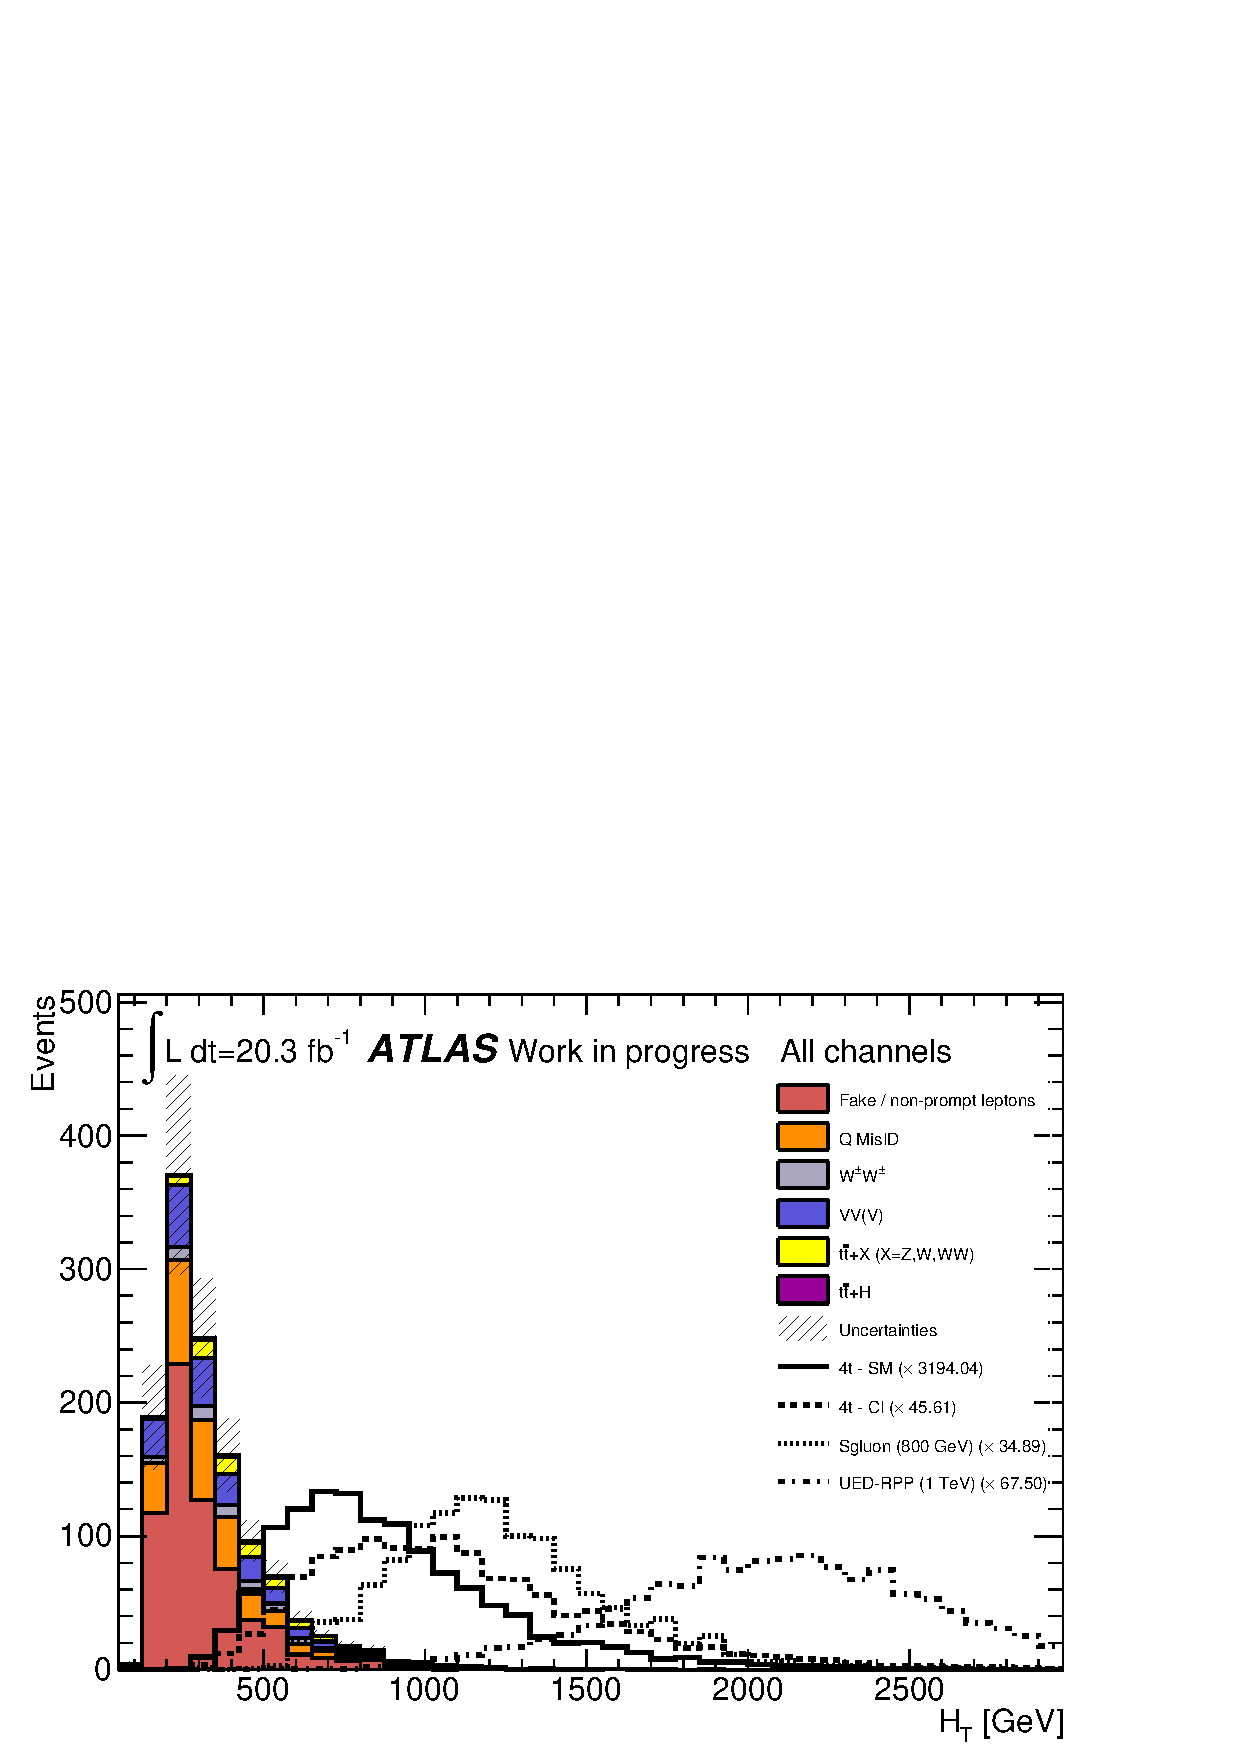
\includegraphics[width=0.48\linewidth]{figures/STD_END_SELECTION_alladded_HT_alladded.pdf}
%\includegraphics[width=0.45\linewidth]{Figures/Optimisations/Categorisation/Motivations/STD_END_SELECTION_alladded_MET_alladded.eps}
%\includegraphics[width=0.45\linewidth]{Figures/Optimisations/Categorisation/Motivations/STD_END_SELECTION_alladded_Nbjets_alladded.eps}
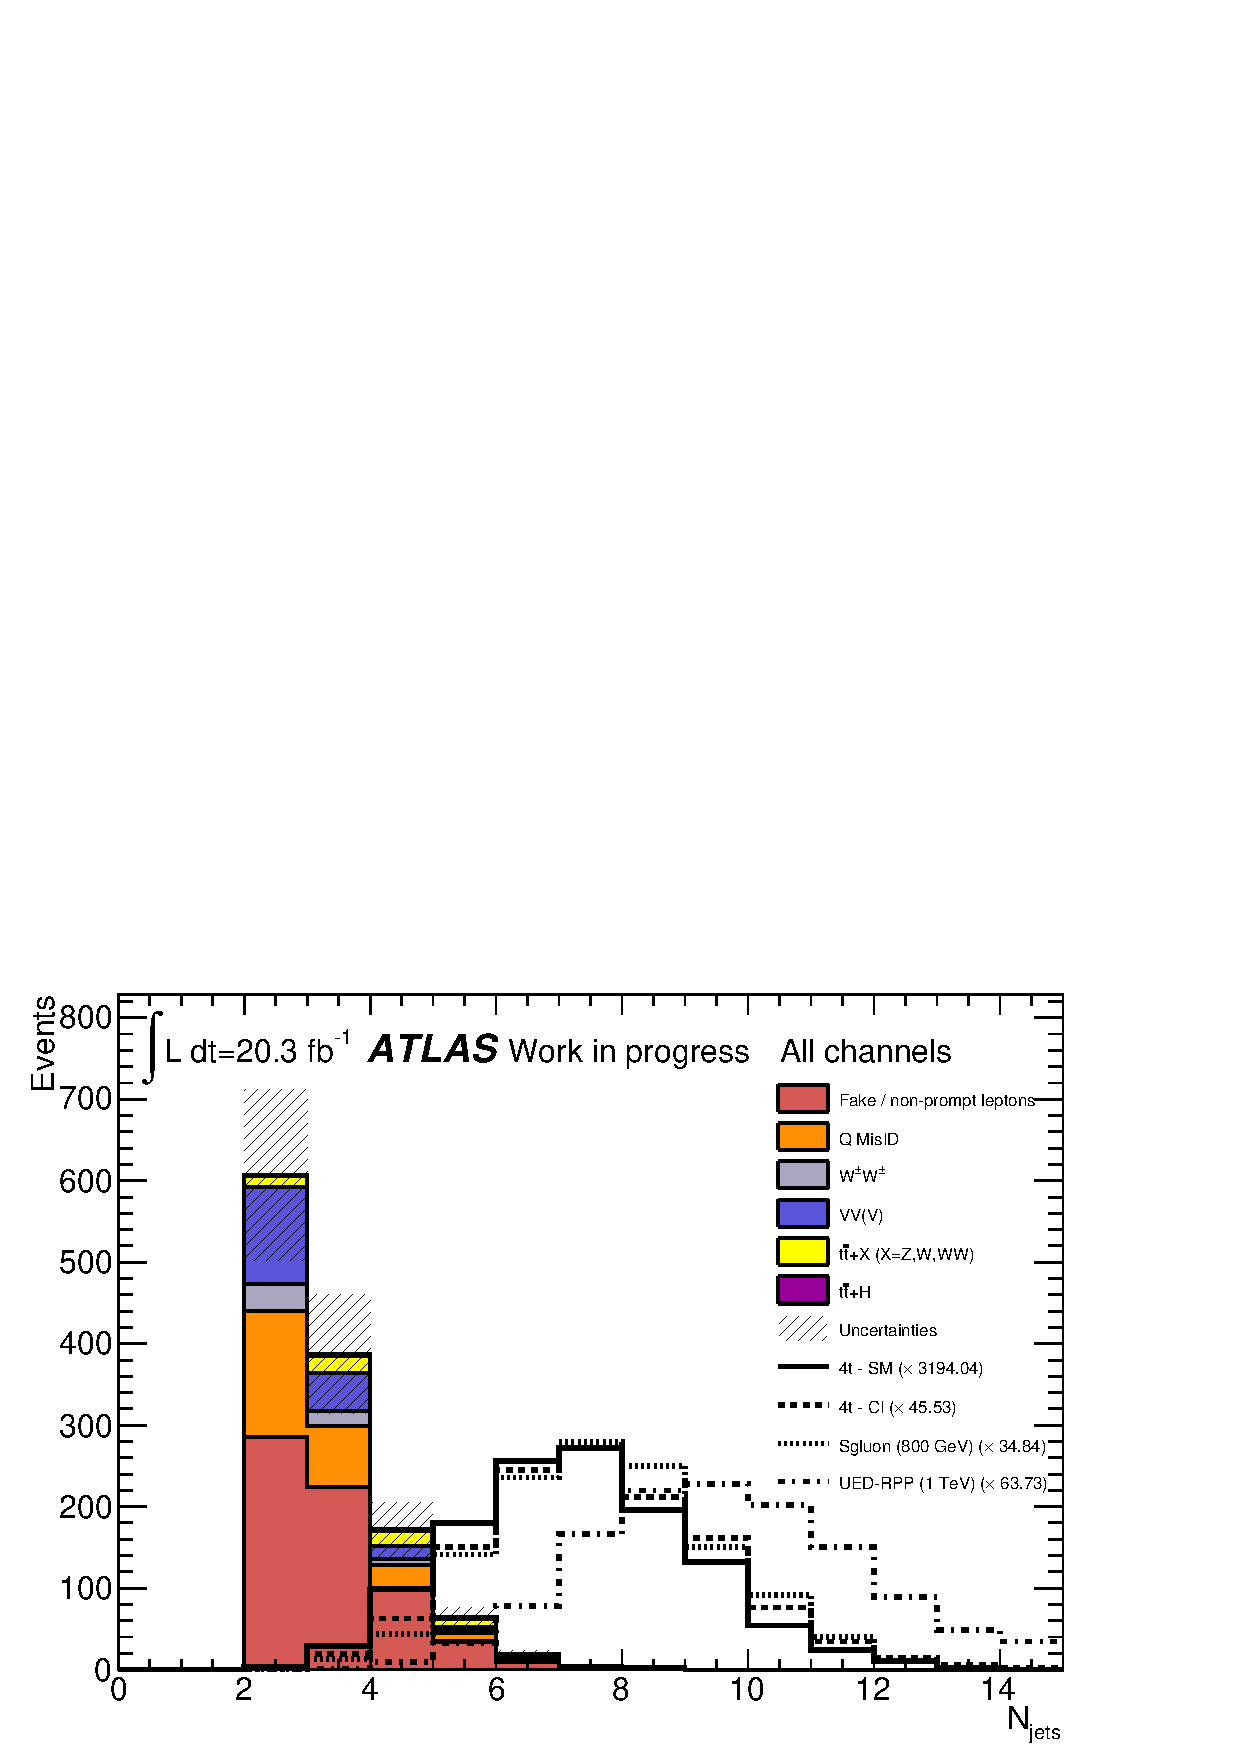
\includegraphics[width=0.48\linewidth]{figures/STD_END_SELECTION_alladded_Njets_alladded.pdf}
\end{center}
\vspace*{-0.5cm}
\caption{Distribution de l'impulsion transverse totale $H_T$ et du nombre de jets par \'ev\'enement pour les diff\'erents signaux \fourtop{} et pour le bruit de fond. Les canaux leptoniques sont ajout\'es.}
\label{fig:opt:cat:distrib_var_4tops}
\end{figure}

Une fois les coupures pr\'ec\'edentes appliqu\'ees, une cat\'egorisation des \'ev\'enements permettant de d\'efinir cinq r\'egions de signal est r\'ealis\'ee. Celles-ci sont pr\'esent\'ees dans la table~\ref{tab:allSR}. Les limites d'exclusion donn\'ees ci-dessous sont obtenues, pour tous les signaux, en combinant ces cinq cat\'egories.

\begin{table*}[!htb]
	\begin{center}
	\begin{tabular}{ c | c | c | c }
	\hline
	\multicolumn{3}{c|}{D\'efinition} & Nom \\
        \hline
	\multirow{2}{*}{$400~< H_T < 700~\GeV{}$}		& \multicolumn{2}{c|}{$N_b = 2$} &  SR4t0 \\
	\cline{2-4}
	 				& \multicolumn{2}{c|}{$N_b \geq 3$} &SR4t1 \\
	\hline
	\multirow{3}{*}{$H_T \geq 700~\GeV$} 			& \multirow{2}{*}{$N_b = 2$}  				& $40~< \hbox{\met} < 100~\GeV$ 		&  SR4t2 \\
	\cline{3-4}
											 &					 				& $\hbox{\met}\geq 100~\GeV$					&  SR4t3 \\
	\cline{2-4}
											&  \multicolumn{2}{c|}{$N_b \geq 3$} & SR4t4 \\
	\hline
\end{tabular}
\caption{D\'efinitions des r\'egions de signal.\label{tab:allSR}}
\end{center}
\end{table*} 

Les bruits de fond consid\'er\'es dans cette analyse sont de deux types :
\begin{maliste}
\item Bruits de fond physiques : il s'agit des processus du mod\`ele standard conduisant \`a la production de deux leptons de m\^eme charge ou de trois leptons. Les processus consid\'er\'es sont ceux dont les \'etats finaux sont $t\bar{t}W$, $t\bar{t}Z$, $t\bar{t}WW$, $WW$, $WZ$, $ZZ$, $t\bar{t}H$, $WH$, $ZH$, $WWW^*$, $ZWW^*$, $tWZ$ et $tH$.
\item Bruits de fond instrumentaux : il s'agit d'\'ev\'enements dans lesquels des objets sont soit mal identifi\'es soit mal reconstruits et qui de ce fait passent les coupures de s\'election. Ces \'ev\'enements sont de deux types. Le premier correspond \`a des \'ev\'enements dans lesquels un ou plusieurs jets sont reconstruits comme des leptons (ce bruit de fond sera d\'enomm\'e \english{fakes} par la suite). Le deuxi\`eme correspond \`a des \'ev\'enements avec deux leptons de charges oppos\'ees dans lesquels la charge de l'un d'entre eux est mal reconstruite (ce bruit de fond sera d\'enomm\'e \english{mis-id} par la suite).
\end{maliste}

Les bruits de fond physiques sont estim\'es gr\^ace \`a la simulation Monte Carlo. Les incertitudes syst\'ematiques consid\'er\'ees sont les incertitudes th\'eoriques sur les sections efficace de production, les incertitudes li\'ees aux radiations dans les \'etats initiaux et finaux, l'incertitude sur la luminosit\'e, les incertitudes sur les efficacit\'es d'identification et la r\'esolution des jets et des leptons et l'incertitude sur l'efficacit\'e d'identification des jets provenant de quarks $b$.

Les bruits de fond instrumentaux sont estim\'es sur les donn\'ees. Les incertitudes sur les taux de mauvaise identification des jets et de mauvaise reconstruction de la charge \'electrique ont \'et\'e estim\'es et pris en compte dans les calculs de limite d'exclusion.

\subsection{R\'esultats}
\label{sec:resultatsAnalyseFourTops}

Les nombres d'\'ev\'enements observ\'es et attendus pour les bruits de fond et le signal dans les cinq r\'egions de signal sont donn\'es dans la table~\ref{tab:allYields} et montr\'es sur la figure~\ref{fig:yieldsBkgSigPlusSignif} (les septs canaux leptoniques sont additionn\'es). 
Cette figure montre \'egalement les nombres d'\'ev\'enements dans des r\'egions de signal autres que celles d\'ecrites jusqu'ici (SRVLQx). 
Ces r\'egions ne sont pas consid\'er\'ees dans l'analyse pr\'esent\'ee dans ce document et ne sont donc pas d\'etaill\'ees. 
Les deux r\'egions qui contribuent le plus \`a l'acceptance pour la production d'\'ev\'enements \fourtop{} par interaction de contact et par le mod\`ele 2UED/RPP sont de loin les r\'egions SR4t3 et SR4t4. 
Le bruit de fond dominant est le processus $t\bar{t}W/Z$. 
Les deux autres fonds qui contribuent de mani\`ere significative sont les fonds \english{mis-id} et \english{fakes}. 
Le nombre d'\'ev\'enements nominal pr\'edit pour ce dernier est faible mais les incertitudes sont grandes (notamment l'incertitude statistique).
Les limites d'exclusion sont davantage d\'egrad\'ees par ces incertitudes que par les autres fonds dont le nombre d'\'ev\'enements nominal est plus grand mais l'incertitude plus faible.
Pour la production d'\'ev\'enements par le mod\`ele standard, ce sont aussi les r\'egions SR4t3 et SR4t4 qui fournissent le plus de signal mais, contrairement au cas des autres signaux, les autres r\'egions contribuent de mani\`ere non n\'egligeable.

Un bon accord entre la pr\'ediction sous l'hypoth\`ese de bruit de fond et l'observation est obtenu dans toutes les r\'egions, sauf dans SR4t3 et SR4t4 o\`u un exc\`es d'\'ev\'enements est pr\'esent dans les donn\'ees. 

\begin{comment}
\begin{table}[!htb]
  \begin{center}
  \hspace*{-1cm}
  \scalebox{0.9}{    \begin{tabular}{l c | c | c | c |c }
      \cline{2-6}\cline{2-6}
      & {\bf SR4t0} & {\bf SR4t1} & {\bf SR4t2} & {\bf SR4t3} & {\bf SR4t4} \\
      \cline{2-6}
      \multicolumn{6}{c}{\bf 2UED/RPP} \\
      \hline
      \multicolumn{1}{c|}{600~\GeV} & $7,7 \pm 1,3 $ & $5,9 \pm 1,1 $ & $81 \pm 4 $ & $321 \pm 9 $ & $588 \pm 11 $\\
      \multicolumn{1}{c|}{800~\GeV} & $0,08 \pm 0,04 $ & $0,12 \pm 0,05 $ & $6,9 \pm 0,4 $ & $38,7 \pm 0,9 $ & $60,9 \pm 1,0 $\\
      \multicolumn{1}{c|}{1000~\GeV} & $ ( 9 \pm 5) \cdot 10^{-3}  $ & $ ( 5 \pm 5) \cdot 10^{-4}  $ & $0,77 \pm 0,05 $ & $5,02 \pm 0,12 $ & $6,72 \pm 0,13 $\\
      \multicolumn{1}{c|}{1200~\GeV} & $< 1,9 \cdot 10^{-4}$ & $< 1,9 \cdot 10^{-4}$ & $ ( 74 \pm 5) \cdot 10^{-3}  $ & $0,648 \pm 0,014 $ & $0,689 \pm 0.013 $\\
      \hline
      \multicolumn{6}{c}{\bf Mod\`ele standard} \\
      \cline{2-6}
      & $ ( 42,8 \pm 2,1) \cdot 10^{-3}  $ & $ ( 38,8 \pm 2.0) \cdot 10^{-3}  $ & $ ( 25,8 \pm 1.7) \cdot 10^{-3}  $ & $ ( 58,3 \pm 2.7) \cdot 10^{-3}  $ & $ ( 105,7 \pm 3.4) \cdot 10^{-3}  $\\
      \cline{2-6}
      \multicolumn{6}{c}{\bf Interaction de contact ($C/\Lambda^2=-4\pi$~TeV$^{-2}$)} \\
      \cline{2-6}
      & $1,60 \pm 0,10 $                  & $1,26 \pm 0,09 $                  & $1,96 \pm 0,12 $                   & $5,26 \pm 0,20 $                    & $8,88 \pm 0,24 $  \\
      \cline{2-6}
      \multicolumn{6}{c}{\bf Bruits de fond} \\
      \hline

       \multicolumn{1}{c|}{$t\bar{t}t\bar{t}$}     & $0,04\pm 0,00 \pm\ 0,03$ & $0,04\pm 0,00 \pm\ 0,03$ & $0,03\pm 0,00 \pm\ 0,02$ & $0,06\pm 0,00 \pm\ 0,05$ & $0,10\pm 0,00 \pm\ 0,08$\\
       \multicolumn{1}{c|}{WZ/ZZ}                        & $0,88\pm 0,19 \pm\ 0,25$ & $0,07\pm 0,12 \pm\ 0,05$ & $0,30\pm 0,14 \pm\ 0,10$ & $0,02\pm 0,12 \pm\ 0,02$ & $0,00\pm 0,12 \pm\ 0,00$\\
       \multicolumn{1}{c|}{$W^{\pm}W^{\pm}$}      & $0,07\pm 0,02 \pm\ 0,02$ & $0,00\pm 0,01 \pm\ 0,00$ & $0,03\pm 0,01 \pm\ 0,02$ & $0,02\pm 0,01 \pm\ 0,02$ & $0,00\pm 0,01 \pm\ 0,00$\\
       \multicolumn{1}{c|}{$t\bar{t}W/Z$}           & $12,60\pm 0,28 \pm\ 4,86$ & $1,24\pm 0,09 \pm\ 0,49$ & $1,87\pm 0,09 \pm\ 0,73$ & $2,46\pm 0,11 \pm\ 0,98$ & $0,57\pm 0,05 \pm\ 0,23$\\
       \multicolumn{1}{c|}{$t\bar{t}WW$}          & $0,20\pm 0,01\pm\ 0,06$ & $0,02\pm 0,00\pm\ 0,01$ & $0,04\pm 0,00\pm\ 0,01$ & $0,09\pm 0,01\pm\ 0,03$ & $0,02\pm 0,00\pm\ 0,01$\\
       \multicolumn{1}{c|}{$t\bar{t}H$}              & $1,79\pm 0,09\pm\ 0,23$ & $0,26\pm 0,03\pm\ 0,05$ & $0,31\pm 0,04\pm\ 0,05$ & $0,44\pm 0,04\pm\ 0,06$ & $0,08\pm 0,02\pm\ 0,02$\\
       \multicolumn{1}{c|}{Triboson}                   & $0,00\pm 0,00\pm\ 0,00$ & $0,00\pm 0,00\pm\ 0,00$ & $0,00\pm 0,00\pm\ 0,00$ & $0,00\pm 0,00\pm\ 0,00$ & $0,00\pm 0,00\pm\ 0,00$\\
       \multicolumn{1}{c|}{VH}                             & $0,02\pm 0,03\pm\ 0,01$ & $0,00\pm 0,08\pm\ 0,00$ & $0,00\pm 0,08\pm\ 0,00$ & $0,00\pm 0,08\pm\ 0,00$ & $0,00\pm 0,08\pm\ 0,00$\\
       \multicolumn{1}{c|}{tX}                               & $0,49\pm 0,02\pm\ 0,07$ & $0,04\pm 0,01\pm\ 0,01$ & $0,09\pm 0,01\pm\ 0,01$ & $0,08\pm 0,01\pm\ 0,01$ & $0,02\pm 0,00\pm\ 0,00$\\
       \multicolumn{1}{c|}{Fakes}                      & $8,61\pm 2,34\pm\ 5,02$ & $1,17\pm 0,82\pm\ 0,68$ & $1,03\pm 0,97\pm\ 0,60$ & $0,00\pm 1,02\pm\ 0,00$ & $0,04\pm 0,83\pm\ 0,02$\\
       \multicolumn{1}{c|}{Mis-Id}                   & $15,07\pm 0,55\pm\ 3,52$ & $0,74\pm 0,11\pm\ 0,18$ & $1,17\pm 0,16\pm\ 0,38$ & $1,09\pm 0,14\pm\ 0,34$ & $0,30\pm 0,09\pm\ 0,10$\\
\hdashline
       \multicolumn{1}{c|}{Total}               & $39,76 \pm 2,43\pm\ 7,26 $ & $3,57 \pm 0,85\pm\ 0,84 $ & $4,86 \pm 1,00\pm\ 1,01 $ & $4,25 \pm 1,05\pm\ 1,07 $ & $1,12 \pm 0,85\pm\ 0,28 $\\

      \hline
       \multicolumn{6}{c}{\bf Observ\'e} \\ \cline{2-6}
                                      & 54 & 6 & 6 & 12 & 6 \\ \cline{2-6}
    \end{tabular}}
    \caption{Nombre d'\'ev\'enements attendu pour les bruits de fond et les signaux recherchés et nombre d'événement observé dans les diff\'erentes r\'egions de signal. Les incertitudes sur les nombres d'\'ev\'enements pour les signaux sont les incertitudes statistiques. Pour les bruits de fond, les premi\`eres et deuxi\`emes incertitudes sont respectivement les incertitudes statistiques et syst\'ematiques (ces derni\`eres sont donn\'ees par l'\'ecart-type de la distribution marginale du nombre d'\'ev\'enements). Pour la production par interaction de contact, les valeurs ont \'et\'e obtenus avec $C/\Lambda^2=-4\pi$~TeV$^{-2}$.\label{tab:allYields}}
  \end{center}
\end{table}
\end{comment}

\begin{table}[!htb]
  \begin{center}
%  \hspace*{-1.cm}
  \scalebox{0.75}{    \begin{tabular}{|l | c | c | c | c |c | }
      \cline{2-6}%\cline{2-6}
       \multicolumn{1}{c|}{ } & {\bf SR4t0} & {\bf SR4t1} & {\bf SR4t2} & {\bf SR4t3} & {\bf SR4t4} \\ \cline{2-6}
       \multicolumn{6}{c}{\bf Signaux} \\
      \hline
      $m_{KK}=600$~\GeV & $7,7 \pm 1,3 $ & $5,9 \pm 1,1 $ & $81 \pm 4 $ & $321 \pm 9 $ & $588 \pm 11 $\\
      $m_{KK}=800$~\GeV & $0,08 \pm 0,04 $ & $0,12 \pm 0,05 $ & $6,9 \pm 0,4 $ & $38,7 \pm 0,9 $ & $60,9 \pm 1,0 $\\
      $m_{KK}=1000$~\GeV & $ ( 9 \pm 5) \cdot 10^{-3}  $ & $ ( 5 \pm 5) \cdot 10^{-4}  $ & $0,77 \pm 0,05 $ & $5,02 \pm 0,12 $ & $6,72 \pm 0,13 $\\
      $m_{KK}=1200$~\GeV & $< 1,9 \cdot 10^{-4}$ & $< 1,9 \cdot 10^{-4}$ & $ ( 74 \pm 5) \cdot 10^{-3}  $ & $0,648 \pm 0,014 $ & $0,689 \pm 0.013 $\\
\hline
 Mod\`ele standard   & $ ( 42,8 \pm 2,1) \cdot 10^{-3}  $ & $ ( 38,8 \pm 2.0) \cdot 10^{-3}  $ & $ ( 25,8 \pm 1.7) \cdot 10^{-3}  $ & $ ( 58,3 \pm 2.7) \cdot 10^{-3}  $ & $ ( 105,7 \pm 3.4) \cdot 10^{-3}  $\\
      \hline
      Interaction contact & $1,60 \pm 0,10 $                  & $1,26 \pm 0,09 $                  & $1,96 \pm 0,12 $                   & $5,26 \pm 0,20 $                    & $8,88 \pm 0,24 $  \\
      \hline
      \multicolumn{6}{c}{\bf Bruits de fond} \\
      \hline

       $t\bar{t}W/Z$            & $12.6 \pm 0.3 \pm 5.4$       & $1.24 \pm 0.09\pm 0.53$& $1.87 \pm 0.09\pm 0.80$ & $2.46 \pm 0.11\pm 1.06$ & $0.57\pm 0.05 \pm 0.25$ \\
      $t\bar{t}H$                & $1.8 \pm 0.1 \pm 0.2$           & $ 0.26 \pm 0.03 \pm 0.05$&  $0.31 \pm 0.04\pm 0.05$ & $0.44\pm 0.04\pm 0.06$ & $0.08\pm 0.02\pm 0.02$\\
       Dibosons                    & $0.95 \pm 0.19\pm 0.25$       & $0.07 \pm 0.12 \pm 0.05$ & $0.33\pm 0.14\pm 0.10$ & $0.04\pm 0.12\pm 0.03$ & $0.00\pm 0.12\pm 0.00$ \\
       Fake/Non-prompt   & $8.61 \pm 2.34 \pm 5.02$ & $1.17 \pm 0.82 \pm 0.68$&  $1.03\pm 0.97 \pm 0.60$ & $0.00\pm 1.02 \pm 0.28$ & $0.04\pm 0.83 \pm 0.24$\\    
       Q mis-Id                    & $15.1 \pm 0.6 \pm 3.5$           & $0.74 \pm 0.11 \pm 0.18$&  $1.17\pm 0.16 \pm 0.38$ & $1.09\pm 0.14 \pm 0.34$ & $0.30\pm 0.09 \pm 0.10$\\  
      Autres                        & $0.75 \pm 0.04 \pm 0.10$      & $0.10 \pm 0.08 \pm 0.03$ &  $0.16\pm 0.08\pm 0.02$ & $0.23\pm 0.08\pm 0.05$ & $0.14\pm 0.08\pm 0.08$\\        
\hdashline
       Total               & $40.0 \pm 2.4 \pm 7.3 $ & $3.6 \pm 0.9 \pm 0.8$ & $4.9 \pm 1.0 \pm 1.0 $ & $4.3 \pm 1.1 \pm 1.1 $ & $1.1 \pm 0.9 \pm 0.4 $\\

      \hline
       \multicolumn{6}{c}{\bf Observ\'e} \\ \cline{2-6}
       \multicolumn{1}{c|}{}                         & 54 & 6 & 6 & 12 & 6 \\ \cline{2-6}
    \end{tabular}}
    \caption{Nombre d'\'ev\'enements attendu pour les signaux recherchés et les bruits de fond et nombre d'événements observés dans les diff\'erentes r\'egions de signal. Les incertitudes sur les nombres d'\'ev\'enements pour les signaux sont les incertitudes statistiques. Pour les bruits de fond, les premi\`eres et deuxi\`emes incertitudes sont respectivement les incertitudes statistiques et syst\'ematiques (ces derni\`eres sont donn\'ees par l'\'ecart-type de la distribution marginale du nombre d'\'ev\'enements). Pour la production par interaction de contact, les nombres donn\'es ont \'et\'e obtenus avec $C/\Lambda^2=-4\pi$~TeV$^{-2}$.\label{tab:allYields}}
  \end{center}
\end{table}

\begin{figure}[!htb]
\begin{center}
\vspace*{-0.5cm}
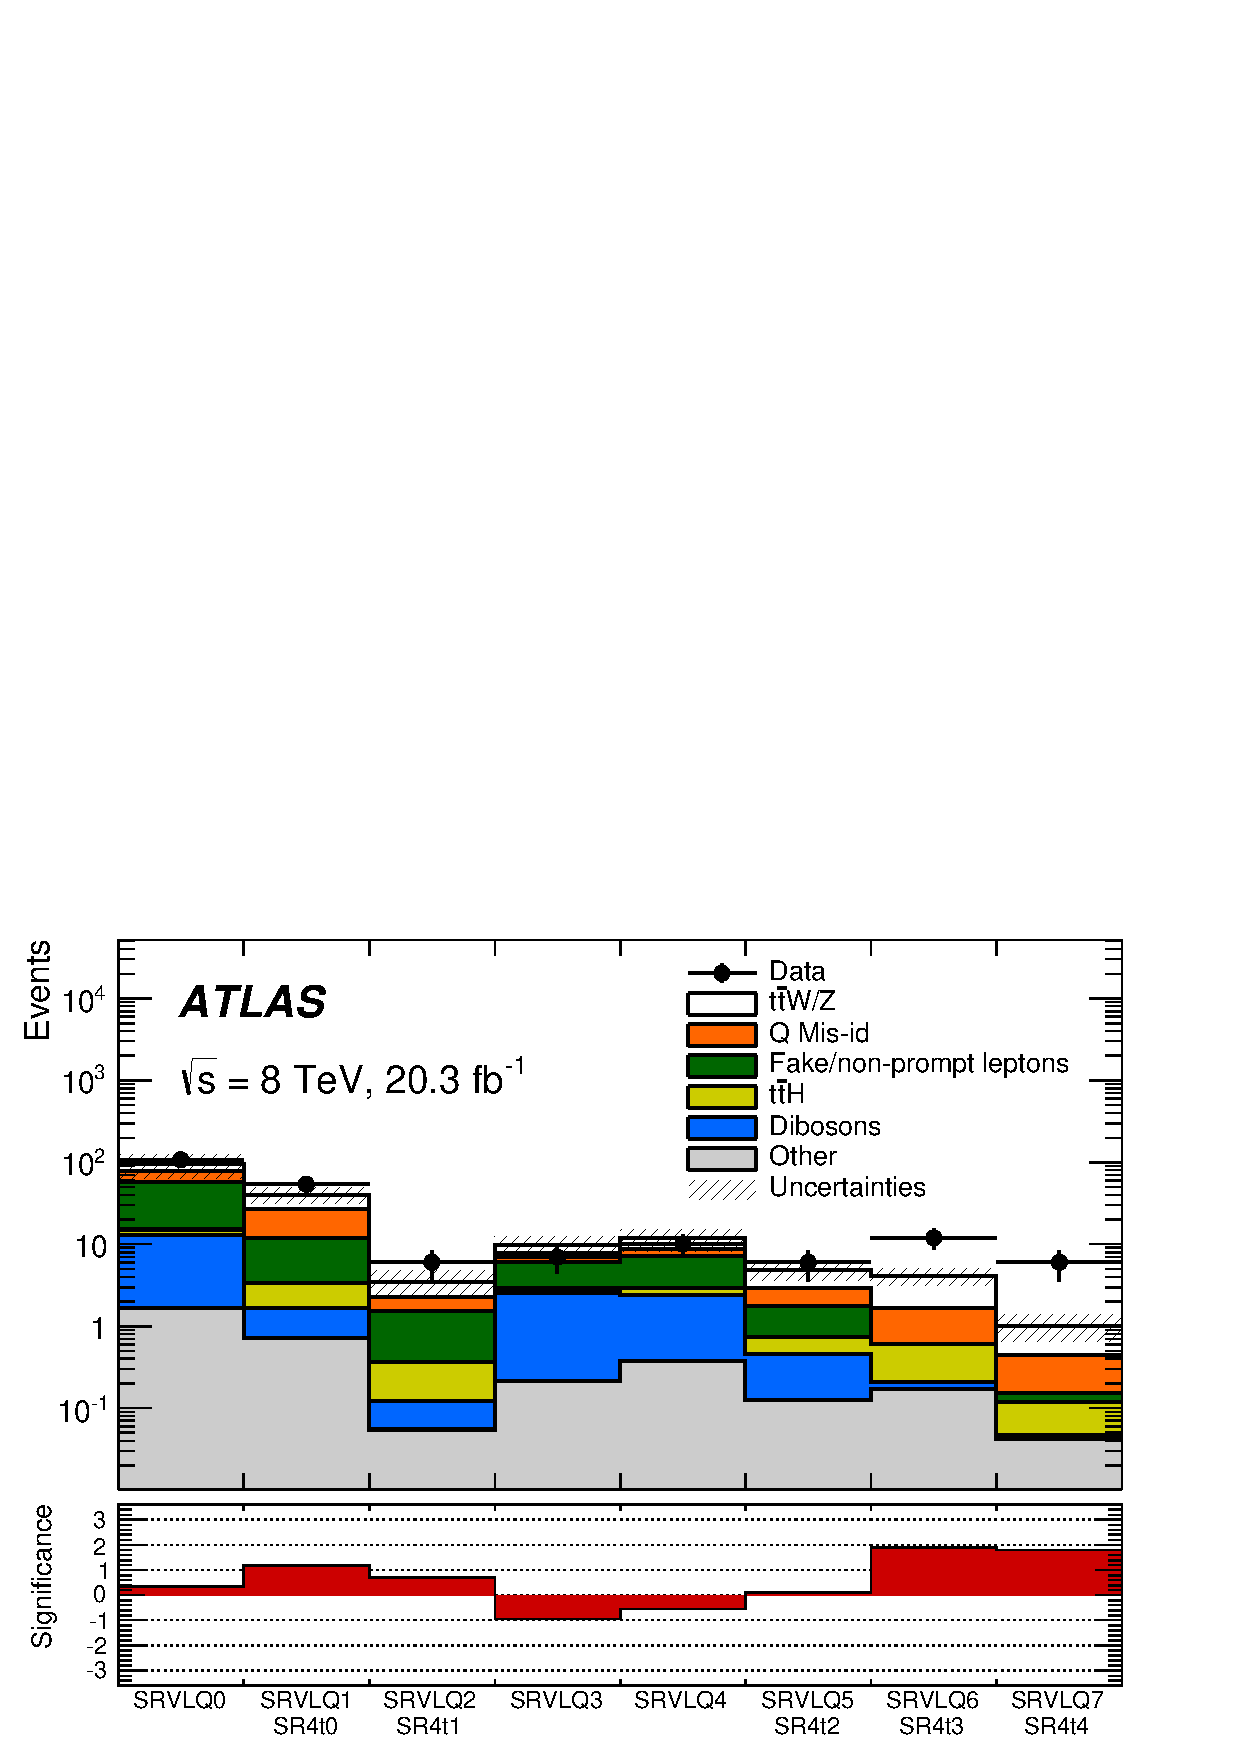
\includegraphics[width=0.65\linewidth]{figures/paperSameSign/ExpectedBackgroundObeservedCategories.pdf}
\end{center}
\vspace*{-0.3cm}
\caption{Nombre d'\'ev\'enements de bruit de fond attendus et observ\'es (en haut) et significance de l'observation (en bas) dans les diff\'erentes r\'egions de signal.}
\label{fig:yieldsBkgSigPlusSignif}
\end{figure}

La significance de l'exc\`es est quantifi\'ee en calculant la \pval~de l'observation sous l'hypoth\`ese de bruit de fond, par la suite not\'ee $p$. 
Celle-ci est dans une tr\`es bonne approximation \'egale \`a $1-\CLb$. 
Elle est traduite en significance par l'expression
\[Z=\Phi^{-1}\left(1-p\right)\]
o\`u $\Phi$ est la fonction de r\'epartition de la distribution normale centr\'ee r\'eduite. 
La significance dans SR4t3 et SR4t4 est tr\`es l\'eg\`erement inf\'erieure \`a $2\sigma$, comme le montre le graphique du bas sur la figure~\ref{fig:yieldsBkgSigPlusSignif}. 
Il s'agit donc d'un exc\`es mod\'er\'e.
Les donn\'ees de cette analyse ont par cons\'equent \'et\'e utilis\'ees pour contraindre les mod\`eles de nouvelle physique consid\'er\'es. 

Les limites d'exclusion sont calcul\'ees avec la m\'ethode hybride fr\'equentiste-bay\'esienne d\'ecrite dans les chapitres~\ref{chap:interpretationStatLimit} et \ref{chap:OTHandTIFOSI}. 
Les cinq r\'egions de signal sont combin\'ees (chacune d'elle correspond \`a un canal $c$ dans l'\'equation~\ref{eq:fullLhoodOTH}). 
%Le programme utilis\'e pour calculer les limites d'exclusion officielles est \mclimit. 
Les distributions \prior~pour les incertitudes statistiques sont gaussiennes et l'interpolation et extrapolation nomm\'ee \text{"}\mclimit\text{"} dans la section~\ref{sec:OTHTreatmentSystUncerts} a \'et\'e utilis\'ee. 
Toutes les limites pr\'esent\'ees dans la suite ont \'et\'e calcul\'ees avec le programmes \mclimit{} et \opthylic. Un excellent accord a \'et\'e trouv\'e \`a chaque fois.

Les limites d'exclusion \`a $95\%$~CL sur les sections efficaces de production d'\'ev\'enements \fourtop{} par interaction de contact et par le mod\`ele standard sont montr\'ees dans la table \ref{tab:limitsExpObsSMCI}. Comme nous l'avons dit dans la section~\ref{sec:interactionContact}, l'\'etablissement d'une limite d'exclusion sur la section efficace de production d'\'ev\'enements \fourtop{} par interaction de contact permet d'exclure certaines r\'egions du plan $\left(C,\Lambda\right)$. Les limites d'exclusion dans ce plan sont montr\'ees sur la figure~\ref{fig:Limit4tCIRPP_20fbObs}(a).

\begin{table}[!htb]
  \begin{center}
    \begin{tabular}{l|c|c | c}
      \hline
      & attendu \`a $1\sigma$ & attendu m\'ediane & observ\'ee\\
      \hline
      Mod\`ele standard   & $\left[18-41\right]$ & $27$ & $70$ \\
      Interaction contact & $\left[16-34\right]$ & $22$  & $61$ \\
      \hline      
    \end{tabular}
    \caption{Limites attendues et observ\'ees sur les sections efficaces de production d'\'ev\'enements \fourtop{} par interaction de contact et par le mod\`ele standard (en fb).}\label{tab:limitsExpObsSMCI}
  \end{center}
\end{table}

\begin{figure}
\centering
\vspace*{-0.5cm}
%\includegraphics[width=0.54\linewidth]{figures/Limit4tCI_20fbObs.pdf}
\includegraphics[width=0.49\linewidth]{figures/paperSameSign/Limit4tCI_20fbObs.pdf}
%\subfloat[toto]{\includegraphics[scale=0.5]{figures/paperSameSign/Limit4tCI_20fbObs.pdf}}
%\includegraphics[width=0.57\linewidth]{figures/RPP_observed_1D11.pdf}
\includegraphics[width=0.49\linewidth]{figures/paperSameSign/RPP_observed_1D11.pdf}
%\subfloat[tata]{\includegraphics[scale=0.5]{figures/paperSameSign/RPP_observed_1D11.pdf}}
%\vspace*{-0.5cm}
\put(-325,-10){$(a)$}
\put(-100,-10){$(b)$}
\caption{Limites d'exclusion attendues et observ\'ee \`a 95\% CL sur la constante $C$ en fonction de l'\'echelle en \'energie $\Lambda$ pour la production d\'ev\'enements \fourtop{} par interaction de contact (\`a gauche) et sur la section efficace de production d'\'ev\'enements \fourtop{} par le mod\`ele 2UED/RPP en fonction de $m_{KK}$ (\`a droite). \label{fig:Limit4tCIRPP_20fbObs}}
\end{figure}

Les limites d'exclusion attendues et observ\'ees en fonction de $m_{KK}$ pour le signal 2UED/RPP sont montr\'ees sur la figure~\ref{fig:Limit4tCIRPP_20fbObs}(b). La section efficace th\'eorique est \'egalement montr\'ee. La limite inf\'erieure attendue m\'ediane (observ\'ee) sur $m_{KK}$ est de 1,05~\TeV{} (0,96~\TeV). Ces limites sont, comme nous l'avons vu dans la section~\ref{sec:modele2UED/RPP}, d\'etermin\'ees en faisant l'hypoth\`ese que les rayons $R_4$ et $R_5$ sont \'egaux ($\xi=1$). Au premier ordre, la section efficace de production ainsi que la cin\'ematique des \'ev\'enements provenant de l'\'etage $\left(1,1\right)$ ne d\'epend que de 
\[\sqrt{\frac{1}{R_4^2}+\frac{1}{R_5^2}}=m_{KK}\sqrt{1+\xi^2}\]

Les limites obtenues sur $m_{KK}$ pour $\xi=1$ peuvent donc \^etre utilis\'ees pour mettre des limites sur $m_{KK}$ pour des valeurs diff\'erentes de $\xi$. La figure~\ref{fig:RPP_observed_2D} montre les limites d'exclusion attendues et observ\'ees dans le plan $\left(\xi,m_{KK}\right)$. Les contraintes cosmologiques sont \'egalement montr\'ees. 

\begin{figure}[!htb]
\begin{center}
\vspace*{-1cm}
%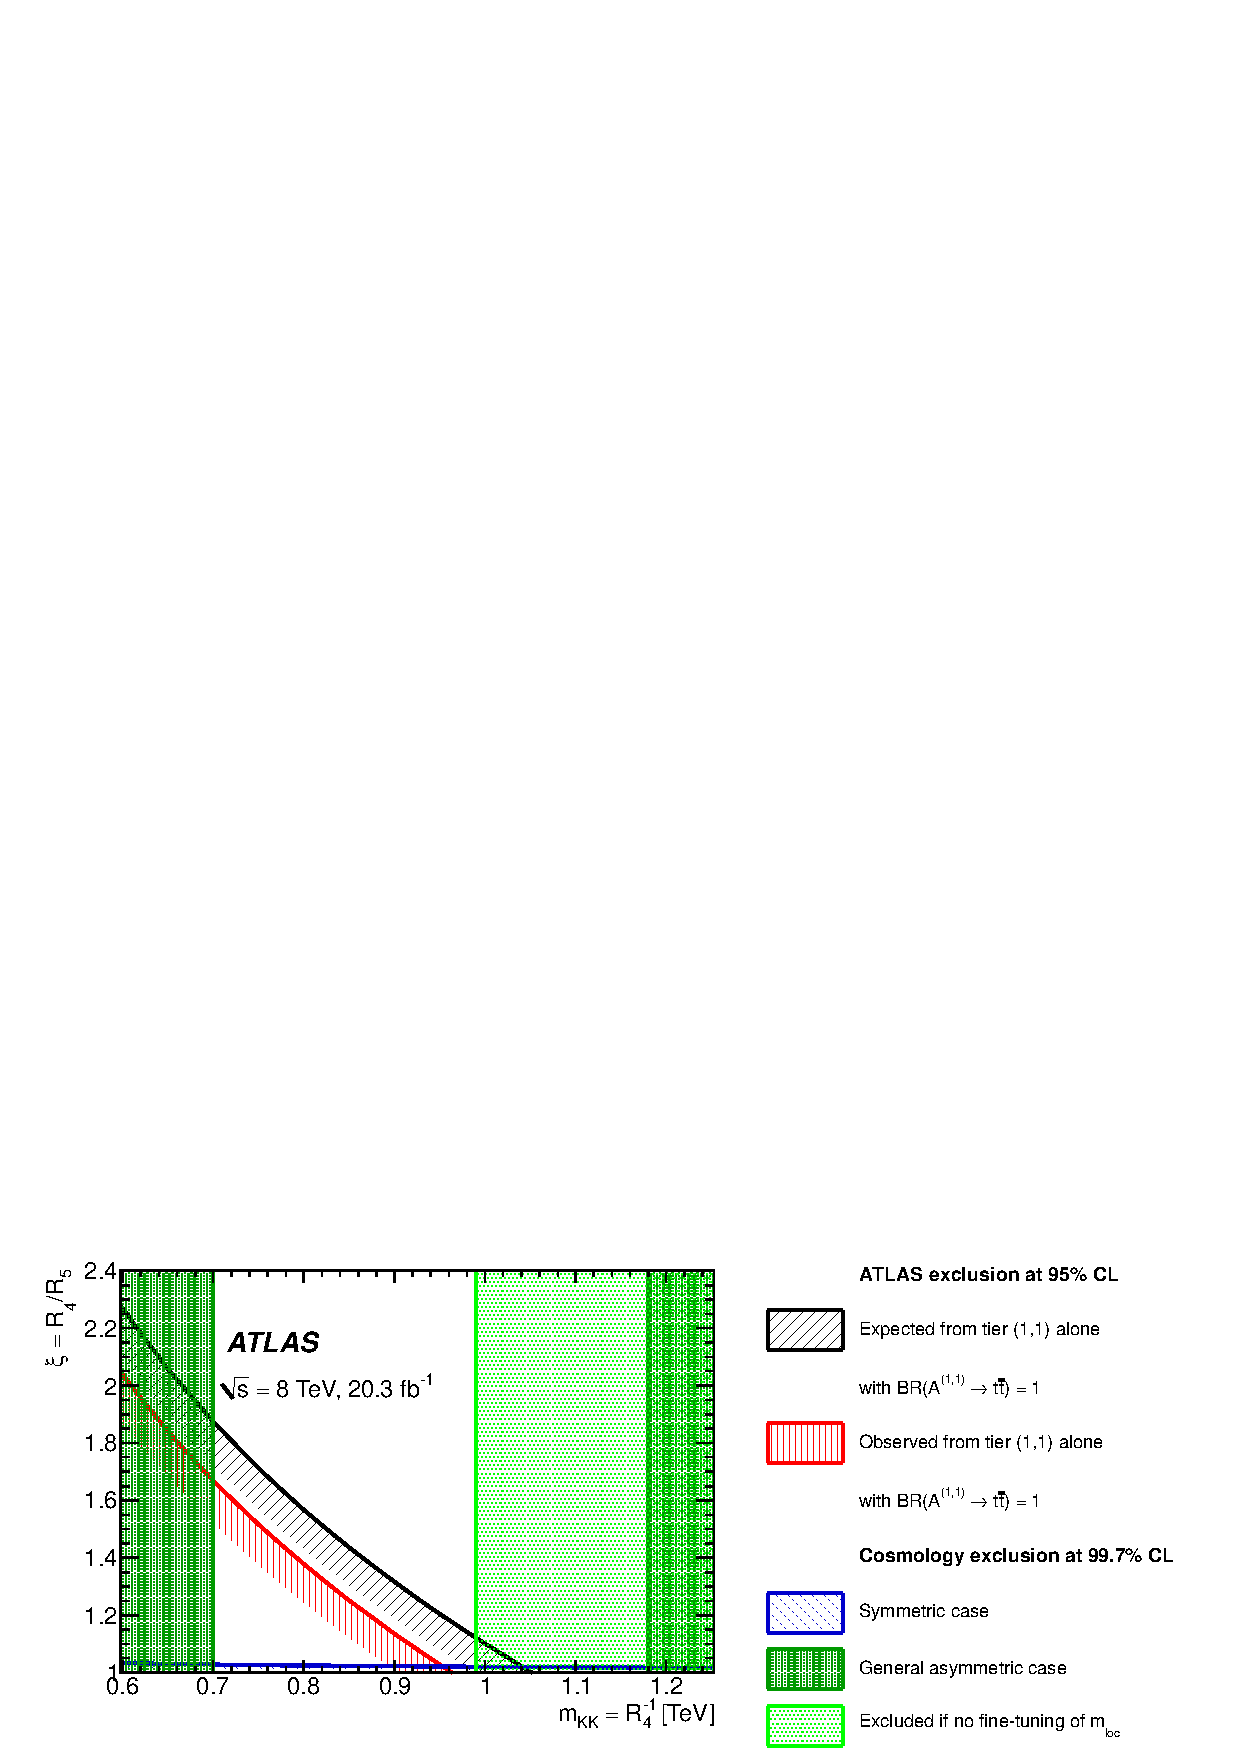
\includegraphics[scale=0.8]{figures/RPP_observed_2D.pdf}
\includegraphics[scale=0.5]{figures/paperSameSign/RPP_observed_2D_snapshotfrompaper.pdf}
\end{center}
\vspace*{-2.5cm}
\caption{Limites d'exclusion attendue et observ\'ee \`a 95\% CL sur $\xi$ en fonction de $m_{KK}$ pour le mod\`ele 2UED/RPP. Les contraintes cosmologiques sont \'egalement montr\'ees.}
\label{fig:RPP_observed_2D}
\end{figure}
%\clearpage

La figure~\ref{fig:Limit4tCIRPP_20fbObs} montre que, lorsque toutes les r\'egions de signal sont combin\'ees, la significance de l'observation est sup\'erieure \`a 2$\sigma$. 
Les distributions du test sous l'hypoth\`ese de bruit de fond pour l'interaction de contact et pour le signal 2UED/RPP avec $m_{KK}=1000~$GeV sont montr\'ees sur la figure~\ref{fig:significanceCIRPPWithOTH}. 
Nous en d\'eduisons que la significance est \'egale \`a environ 2,4 pour la production d'\'ev\'enements \fourtop{} par interaction de contact et environ 2,5 pour la production par le mod\`ele 2UED/RPP avec $m_{KK}=1000~$GeV.

\begin{figure}[!htb]
\begin{center}
\includegraphics[width=0.43\linewidth]{macros/significanceContactInteractionMcLimitNormal.pdf}
\includegraphics[width=0.43\linewidth]{macros/significance2UEDRPPMkk1000McLimitNormal.pdf}
\end{center}
\vspace*{-0.7cm}
\caption{Distribution du test statistique $\qmu$ sous l'hypoth\`ese de bruit de fond pour la production d'\'ev\'enements \fourtop{} par interaction de contact (\`a gauche) et par le mod\`ele 2UED/RPP avec $m_{KK}=1000$~GeV. La valeur observ\'ee $\qmuobs$ est repr\'esent\'ee par la ligne verticale. La \pval~$p$ et la significance $Z$ de l'observation sont \'egalement donn\'ees.\label{fig:significanceCIRPPWithOTH}}
\end{figure}

Ces valeurs de significance montrent que la diff\'erence entre l'observation et la pr\'ediction commence \`a \^etre significative lorsque toutes les r\'egions de signal sont combin\'ees. 
Plusieurs v\'erifications ont \'et\'e effectu\'ees afin de v\'erifier que cette diff\'erence ne provient pas d'une mauvaise estimation des bruits de fond. 
Pour les fonds $t\bar{t}W/Z$, diff\'erents g\'en\'erateurs et diff\'erents r\'eglages de ces g\'en\'erateurs ont \'et\'e utilis\'es. 
Pour les fonds intrumentaux, il a \'et\'e v\'erifi\'e que les leptons se trouvant dans les r\'egions SR4t3 et SR4t4 ont des propri\'et\'es similaires \`a celles attendues pour des vrais leptons. 
De plus, ces fonds ont \'et\'e estim\'es avec la simulation uniquement. 
Dans tous les cas, les nombres d'\'ev\'enements obtenus dans les diff\'erentes r\'egions de signal sont compatibles avec ceux issus de l'estimation nominale.

% La figure~\ref{} montre les distributions des variables $H_T$ et du nombre de jets

\begin{comment}
\blabla contribution des diff\'erentes categories a la sensibilite\\
\\
\blabla bkg pour 2lep et 3leps\\
\\
\blabla exces -> commenter (mettre plot pValue)


\subsection{V\'erification avec \opthylic}

Toutes les limites d'exclusion pour les signaux consid\'er\'es dans ce chapitre ont \'et\'e v\'erifi\'ees avec \opthylic. Un bon accord entre \mclimit{} et \opthylic~a \'et\'e observ\'e. La figure~\ref{fig:ExclusionPlot_RPPFullStat_OTHVsBayesian} montre les r\'esultats obtenus avec ces deux programmes dans le cas du signal 2UED/RPP.

\begin{figure}[!htb]
\begin{center}
\includegraphics[width=0.54\linewidth]{macros/ExclusionPlot_RPPFullStat_McLimitVsOTH.pdf}
\end{center}
\caption{Comparaison des limites observ\'ees et attendues calcul\'ees avec \mclimit~et \opthylic~pour le signal 2UED/RPP.}
\label{fig:ExclusionPlot_RPPFullStat_OTHVsBayesian}
\end{figure}

Les significances d'observation ont \'egalement \'et\'e calcul\'ees avec \opthylic. La figure~\ref{fig:significanceCIRPPWithOTH} montre par exemple la distribution du test statistique sous l'hypoth\`ese de bruit de fond ainsi que sa valeur observ\'ee pour la production d'\'ev\'enements par interaction de contact et par le mod\`ele 2UED/RPP. La valeur de $\mu$ utilis\'ee pour calculer le test $\qmu$ est $\mu=1$. Les valeurs de significance sont en très bon accord avec celles trouvées par \mclimit{} et confortent ainsi les r\'esultats obtenus.

\begin{figure}[!htb]
\begin{center}
\includegraphics[width=0.43\linewidth]{macros/significanceContactInteractionMcLimitNormal.pdf}
\includegraphics[width=0.43\linewidth]{macros/significance2UEDRPPMkk1000McLimitNormal.pdf}
\end{center}
\caption{Distribution du test statistique $\qmu$ sous l'hypoth\`ese de bruit de fond pour la production d'\'ev\'enements \fourtop{} par interaction de contact (\`a gauche) et par le mod\`ele 2UED/RPP avec $m_{KK}=1000$~GeV. La valeur observ\'ee $\qmuobs$ est repr\'esent\'ee par la ligne verticale. La \pval~$p$ et la significance $Z$ de l'observation sont \'egalement donn\'ees.\label{fig:significanceCIRPPWithOTH}}
\end{figure}

\end{comment}

\subsection{Variation d'interpr\'etation}

En plus des v\'erifications d\'ecrites ci-dessus, d'autres \'etudes ont \'et\'e r\'ealis\'ees sur l'interpr\'etation statistique des donn\'ees.
Comme nous l'avons vu dans les chapitre~\ref{chap:interpretationStatLimit} et \ref{chap:OTHandTIFOSI}, toute interpr\'etation statistique contient une part d'arbitraire li\'ee aux choix qui sont faits pour r\'ealiser les calculs (que ce soit les calculs de limite ou de significance). 
Ces choix sont de deux types. Premi\`erement, il y a le choix de l'approche statistique. 
Les r\'esultats publi\'es pr\'esent\'es ci-dessus ont \'et\'e obtenus avec une approche hybride et il est int\'eressant de les comparer \`a ceux obtenus par une approche fr\'equentiste et bay\'esienne. 
Deuxi\`emement, il y a les choix relatifs au traitement des incertitudes statistiques et syst\'ematiques. 
Ces derniers doivent \^etre fait quelque soit l'approche statistique utilis\'ee.
Les sections suivantes pr\'esentent les r\'esultats obtenus en faisant varier ces choix. 
%La robustesse des r\'esultats publi\'es . 

\subsubsection{Interpr\'etation hybride vari\'ee}
\label{sec:variationInterpretationFourTopHybride}

Les limites d'exclusion et significances d'observation ont \'et\'e calcul\'ees avec \opthylic{} en faisant varier l'interpolation et extrapolation des incertitudes syst\'ematiques et les distributions \prior{} pour les incertitudes statistiques. La figure~\ref{fig:interpretationHybrideVariee} montre les limites pour les mod\`eles d'interaction de contact et 2UED/RPP avec $m_{KK}=1000~$GeV obtenues avec la configuration standard pr\'esent\'ee pr\'ec\'edemment et celles obtenues avec une interpolation polynomiale, une extrapolation exponentielle et une distribution \prior{} gamma donn\'ee par la formule~\ref{eq:gammaPriorsInOTH} (une distribution \prior{} $\pi\left(y\right)\propto 1/y$ est utilis\'ee). D'autres comparaisons ont \'et\'e effectu\'ees en changeant d'interpolation/extrapolation et en prenant des distributions \prior{} log-normales. 
Les limites obtenues sont similaires \`a celles obtenues avec la distribution gamma.

\vspace*{-0.5cm}
\begin{center}
\begin{figure}[!htb]
\includegraphics[width=0.45\textwidth]{macros/ExclusionPlot_RPPFullStat_McLimitVsOTHpolyexpo_gammahyper.pdf}
\includegraphics[width=.48\textwidth]{macros/CVsLambdaForContactInteractionMcLimitVsOTHpolyexpogammahyper.pdf}
\caption{Limites observ\'ees et attendues \`a $95\%$ CL pour le mod\`ele 2UED/RPP avec $m_{KK}=1000~$GeV (\`a gauche) et le mod\`ele d'interaction de contact (\`a droite) obtenue avec diff\'erents sch\'emas d'interpolation et extrapolation pour les incertitudes syst\'ematiques et diff\'erentes distributions \prior{} pour les incertitudes statistiques. Les r\'esultats pour l'interpolation et extrapolation nomm\'ee \text{"}\mclimit\text{"} et des distributions \prior{} normales sont montr\'es en vert, jaune et noir et ceux pour l'interpolation polynomiale, l'extrapolation exponentielle et des distributions \prior{} gammas sont montr\'es en gris. \label{fig:interpretationHybrideVariee}}
\end{figure}
\end{center}
\vspace*{-1cm}
Les diff\'erences entre la configuration standard et la configuration vari\'ee sont essentiellement dues au changement dans les distributions \prior{}. Le passage de distributions normales aux distributions gammas (ou log-normales) se traduit par un diminution de la valeur moyenne du nombre d'\'ev\'enements (ceci est vrai sous l'hypoth\`ese de bruit de fond et sous l'hypoth\`ese signal plus bruit de fond). 
La distribution du test est par cons\'equent d\'ecal\'ee vers les grandes valeurs.
De plus, elle est davantage asym\'etrique du fait de l'asym\'etrie de la distribution gamma (ou log-normale) lorsque son esp\'erance est faible. 
Ceci a pour effet de r\'eduire l\'eg\`erement les limites attendues. 
Les limites observ\'ees sont quant \`a elles plus grandes avec des distributions gammas. En effet, l'exc\`es est tel que \CLb{} est tr\`es proche de 1 quelque soient les distributions \prior. Il faut donc un $\mu$ plus grand avec les distributions gammas qu'avec les distributions normales pour atteindre $\CLsb=0,05$. 

Les diff\'erences que nous venons de d\'ecrire se traduisent \'egalement par des diff\'erences dans la significance de l'exc\`es. L'utilisation de distributions gamma (ou log-normale) fait passer la significance de 2,4 \`a 2,7 dans le cas de la production par interaction de contact et de 2,5 \`a 2,8 pour la production par le mod\`ele 2UED/RPP avec $m_{KK}=1000~$GeV. 

Ces \'etudes montrent qu'un changement d'interpr\'etation hybride conduit \`a des variations de 6\% \`a 12\% dans les limites d'exclusion et d'environ 12\% dans les significances.

\subsubsection{Interpr\'etation bay\'esienne}
\label{sec:variationInterpretationFourTopBayesian}

Les limites d'exclusion pour tous les signaux ont \'egalement \'et\'e calcul\'ees par l'approche bay\'esienne avec l'outil \tifosi~(voir section~\ref{sec:tifosi}). Pour tous les r\'esultats pr\'esent\'es ci-dessous, une distribution \prior~uniforme sur le param\`etre d'int\'er\^et $\mu$ a \'et\'e utilis\'ee. Les distributions \prior~pour les incertitudes statistique sont gaussiennes. L'interpolation et l'extrapolation utilis\'ees par le programme \mclimit{} n'\'etant pas disponible dans \tifosi, nous avons choisi l'interpolation polynomiale et l'extrapolation exponentielle d\'ecrites dans le chapitre~\ref{chap:OTHandTIFOSI}. Le niveau de cr\'edibilit\'e des intervalles bay\'esiens est choisi \'egal au niveau de confiance des intervalles hybrides, soit 95\% (rappelons que, dans le cas o\`u un seul canal est consid\'er\'e avec un signal parfaitement connu, l'utilisation d'une m\^eme valeur pour les deux niveaux conduit \`a la m\^eme inf\'erence sur $\mu$).

%Les diff\'erences entre les intervalles hybride et bay\'esien proviennent donc de la combinaison des canaux et de la pr\'esence d'incertitudes sur le nombre d'\'ev\'enement de signal attendu.

Les limites bay\'esienne et hybride (calcul\'ees avec \opthylic) pour les diff\'erents signaux sont donn\'ees dans la table~\ref{tab:comparaisonLimitesHybrideBayesienne}. 
\vspace*{0.5cm}
\begin{table}[!htb]
  \begin{center}
    \begin{tabular}{|c|c|c|c|c|}
      \hline
      \multirow{2}{*}{Signal}                  &  \multicolumn{2}{c|}{Limite attendue}       &  \multicolumn{2}{c|}{Limite observ\'ee}     \\ \cline{2-5}
                                                                    &  hybride              & bay\'esienne           &   hybride     &   bay\'esienne             \\ \hline
      2UED/RPP $m_{KK}=600$ GeV   &   8,67        &    6,98                &      23,0        &    21,8                     \\ \hline
      2UED/RPP $m_{KK}=800$ GeV   &    7,38       &     6,03               &     19,3         &    19,0                     \\ \hline  
      2UED/RPP $m_{KK}=1000$ GeV  &   6,62        &     5,62              &   17,5           &    16,7                  \\ \hline  
      2UED/RPP $m_{KK}=1200$ GeV  &    6,24          &     5,17           &    16,7          &     16,0                    \\ \hline  
      Interaction contact                       &     22,4       &      19,0                             &      61,2         &    66,3                        \\ \hline  
      Mod\`ele standard                        &     26,6     &         21,0                     &         70,1      &     66,7                       \\ \hline  
    \end{tabular}
    \caption{Limites d'exclusion sur la section efficace de production (en fb) pour les diff\'erents signaux consid\'er\'es dans cette analyse. Les limites hybrides (bay\'esiennes) sont calcul\'ees avec le programme \opthylic~\`a 95\% CL (\tifosi~\`a 95\% CI). Les limites bay\'esiennes sont calcul\'ees avec une distribution \prior~uniforme sur le param\`etre d'int\'er\^et. Les limites attendues sont les limites m\'edianes sous l'hypoth\`ese du bruit de fond dans le cas hybride et les limites calcul\'ees avec un échantillon \english{asimov} dans le cas bay\'esien. Pour la production par interaction de contact, les nombres d'\'ev\'enements ont \'et\'e obtenus avec $C/\Lambda^2=-4\pi$~TeV$^{-2}$}\label{tab:comparaisonLimitesHybrideBayesienne}
  \end{center}
\end{table}
\clearpage
Les limites attendues dans le cas bay\'esien sont calcul\'ees avec un \'echantillon \english{asimov}, c'est-\`a-dire, en utilisant les notations des chapitres~\ref{chap:interpretationStatLimit} et \ref{chap:OTHandTIFOSI}, avec
\[\nobsc=\sum\limits_i \bci\]
pour tous les canaux $c$. Les limites attendues bay\'esiennes sont plus faibles que les limites attendues hybrides de 15\% \`a 21\% en fonction du signal. 
Pour tous les signaux, les limites attendues bay\'esiennes se trouvent dans l'intervalle de confiance \`a $\pm 1\sigma$ obtenue dans le cas hybride. 
Les limites observ\'ees sont compatibles \`a 10\% pr\`es.



La figure \ref{fig:ExclusionPlot_RPPFullStatAndCI_OTHVsBayesian} montre les limites hybrides et bayésiennes observ\'ees et attendues pour le signal 2UED/RPP en fonction de $m_{KK}$ (\`a gauche) et pour l'interaction de contact (\`a droite). Les limites observ\'ees et attendues sur $m_{KK}$ sont sensiblement les m\^emes dans les deux cas (elles sont augment\'ees avec le calcul bay\'esien d'environ 16~GeV et 3,5~GeV respectivement). Les r\'egions exclues dans le plan $\left(C,\Lambda\right)$ changent elles-aussi relativement peu. 

\begin{figure}[!htb]
\begin{center}
\includegraphics[width=0.45\linewidth]{macros/ExclusionPlot_RPPFullStat_OTHVsBayesian.pdf}
\includegraphics[width=0.47\linewidth]{macros/CVsLambdaForContactInteractionHybridVsBayesian.pdf}
\end{center}
\caption{Comparaison des limites attendues et observ\'ees bay\'esiennes et hybrides en fonction de $m_{KK}$ pour la production d'\'ev\'enements \fourtop{} par le mod\`ele 2UED/RPP (\`a gauche) et dans le plan $\left(C,\Lambda\right)$ pour la production par interaction de contact (\`a droite).\label{fig:ExclusionPlot_RPPFullStatAndCI_OTHVsBayesian}}
\end{figure}

\subsubsection{Interpr\'etation fr\'equentiste}
\label{sec:fourtopsResultatsFreq}

Les limites et significances ont \'egalement \'et\'e calcul\'ees suivant une m\'ethode purement fr\'equentiste afin d'\^etre compar\'ees aux r\'esultats hybrides et bay\'esiens discut\'es pr\'ec\'edemment. 
Le mod\`ele statisque utilis\'e ici est l\'eg\`erement diff\'erent. 
Nous avons en effet utilis\'e le mod\`ele construit par le programme \histfactory~\cite{Cranmer:1456844} dans le but d'appliquer un traitement similaire \`a celui appliqu\'e habituellement dans ATLAS pour les inf\'erences fr\'equentistes. 
Dans chaque canal, un seul param\`etre de nuisance est introduit pour d\'ecrire les incertitudes statistiques (alors que pr\'ec\'edemment le nombre de param\`etres de nuisance \'etait \'egal au nombre total d'\'echantillons de signal et de bruit de fond) et ce param\`etre est contraint par une distribution de Poisson. 
La figure~\ref{fig:pureFrequentistmKK1000GeVScan} montre \CLsb, \CLb{} et \CLs{} pour plusieurs valeurs de $\mu$ dans le cas du mod\`ele 2UED/RPP avec $m_{KK}=1000~$GeV. Cette figure permet de d\'eterminer la limite observ\'ee et les limites attendues par la deuxi\`eme m\'ethode d\'ecrite dans la section~\ref{sec:limitesAttenduesHypBdf}. 
Les valeurs obtenues sont donn\'ees dans la table~\ref{tab:comparaisonPureFrequentistAsymptotic2UEDRPPmKK1000GeV}. Cette table donne \'egalement les valeurs obtenues en faisant l'approximation asymptotique d\'ecrite dans la section~\ref{sec:limiteAsymptotique}. 

\begin{figure}[!htb]
\begin{center}
\includegraphics[width=0.5\linewidth]{figures/pureFrequentistmKK1000GeVScan.pdf}
\end{center}
\vspace*{-0.3cm}
\caption{\CLs{}, \CLsb{} et \CLb{} en fonction de $\mu$ dans l'interpr\'etation fr\'equentiste pour le mod\`ele 2UED/RPP avec $m_{KK}=1000~$GeV. Les valeurs de \CLs{} observ\'ees, attendues m\'edianes et \`a $-2\sigma, -1\sigma, +1\sigma~\text{et}~+2\sigma$ sont montr\'ees.\label{fig:pureFrequentistmKK1000GeVScan}}
\end{figure}

\begin{table}[!htb]
  \begin{center}
    \begin{tabular}{|c|c|c|c|c|c|c|}
      \cline{2-7}
      \multicolumn{1}{c|}{} & \multicolumn{5}{c|}{Limite attendue}    &   \multirow{2}{*}{Limite observ\'ee}   \\ \cline{2-6}
      \multicolumn{1}{c|}{}  & $-2\sigma$   & $-1\sigma$  & m\'ediane  & $+1\sigma$  & $+2\sigma$ &   \\ \hline
      calcul exact  &  0,29  &  0,39 & 0,55  & 0,81 & 1,22 &  1,60 \\ \hline
      calcul asymptotique  & 0,32   & 0,41  &  0,55 & 0,80 & 1,15 & 1,62 \\ \hline
    \end{tabular}
    \caption{Limites d'exclusion sur $\mu$ pour le signal 2UED/RPP avec $m_{KK}=1000~$GeV. Les valeurs obtenues avec un calcul exact et en faisant l'approximation asymptotique sont donn\'ees.}\label{tab:comparaisonPureFrequentistAsymptotic2UEDRPPmKK1000GeV}
  \end{center}
\end{table}

Les r\'esultats pr\'esent\'es dans la table~\ref{tab:comparaisonPureFrequentistAsymptotic2UEDRPPmKK1000GeV} montrent que l'approximation asymptotique est une bonne approximation pour notre analyse. 
C'est \'egalement ce que montre la figure~\ref{fig:outputObservationSignificance2UEDRPPmKK1000GeV} dans laquelle la distribution du test obtenue par des pseudo-exp\'eriences est compar\'ee \`a la distribution asymptotique sous l'hypoth\`ese de bruit de fond.
Nous avons par cons\'equent utilis\'e la limite asymptotique pour calculer les limites pour les autres valeurs de $m_{KK}$ dans le cas du signal 2UED/RPP et pour la production par interaction de contact. 
Ces calculs sont bas\'es sur l'\'equation~\ref{eq:pureFreqAsymptoticLimit} pour les limites observ\'ees. Pour les limites attendues, $\Est{\mu}$ est remplac\'e dans cette \'equation par $\mu'+N\sigma$ (nous rappelons que $\sigma$ est ici l'\'ecart-type de la distribution de $\Est{\mu}$ dans la limite asymptotique) avec $N=-2, -1, 0, +1, +2$ ~\cite{Armbruster:1553771}. 

\begin{figure}[!htb]
\begin{center}
\includegraphics[width=0.48\linewidth]{figures/outputObservationSignificance2UEDRPPmKK1000GeV.pdf}
\put(-120,150){\footnotesize{2UED/RPP}}
\put(-120,138){\footnotesize{$m_{KK}=1000$~GeV}}
\vspace*{-0.7cm}
\caption{Distribution du test statistique $q_0/2$ sous l'hypoth\`ese de bruit de fond pour le signal 2UED/RPP avec une masse $m_{KK}=1000~$GeV. La distribution attendue dans la limite asymptotique est montr\'ee par la courbe bleue en trait plein.\label{fig:outputObservationSignificance2UEDRPPmKK1000GeV}}
\end{center}
\end{figure}

La figure~\ref{fig:ExclusionPlot_RPPFullStatAndCI_MclimitVsPureFrequentist} compare les limites fr\'equentistes asymptotiques \`a celles obtenues par l'approche hybride dans la section~\ref{sec:resultatsAnalyseFourTops}. 
Les limites fr\'equentiste et hybride ne diff\`erent pas de plus de 10\%. 
Ce r\'esultat, comme ceux pr\'esent\'es dans les sections~\ref{sec:variationInterpretationFourTopHybride} et \ref{sec:variationInterpretationFourTopBayesian}, permet d'avoir une \'evaluation quantitative de la robustesse des limites publi\'ees.
% pr\'esent\'ees dans la section~\ref{sec:resultatsAnalyseFourTops}.
\enlargethispage{0.5cm}
\begin{figure}[!htb]
\begin{center}
\includegraphics[width=0.45\linewidth]{macros/ExclusionPlot_RPPFullStat_McLimitVsAsymptotic.pdf}
\includegraphics[width=0.47\linewidth]{macros/CVsLambdaForContactInteractionHybridVsAsymptotic.pdf}
\end{center}
\vspace*{-0.3cm}
\caption{Comparaison des limites attendues et observ\'ees obtenues par un calcul fr\'equentiste (dans la limite asymptotique) et un calcul hybride en fonction de $m_{KK}$ pour la production d'\'ev\'enements \fourtop{} par le mod\`ele 2UED/RPP (\`a gauche) et dans le plan $\left(C,\Lambda\right)$ pour la production par interaction de contact (\`a droite).\label{fig:ExclusionPlot_RPPFullStatAndCI_MclimitVsPureFrequentist}}
\end{figure}

% Nous avons \'egalement calcul\'e les significances dans l'approche purement fr\'equentiste. La figure~\ref{fig:outputObservationSignificance2UEDRPPmKK1000GeV} montre la distribution du test sous l'hypoth\`ese de bruit de fond. La distribution asymptotique (distribution de chi-carr\'ee) est \'egalement montr\'ee. 


\section{Conclusion}

La recherche d'\'ev\'enements avec quatre quarks top dans les donn\'ees enregistr\'ees par l'exp\'erience ATLAS en 2012 \`a $\sqrt{s}=8$~TeV a \'et\'e pr\'esent\'ee. Les mod\`eles consid\'er\'es permettent de couvrir un nombre relativement important de sc\'enarios de nouvelle physique pr\'edisants ce type d'\'ev\'enements. Un exc\`es d'\'ev\'enements par rapport \`a la pr\'ediction de bruit de fond a \'et\'e observ\'e. Cet exc\`es n'\'etant pas significatif, des limites sup\'erieures sur les sections efficaces de production ont \'et\'e pos\'ees. Ces limites ont ensuite \'et\'e traduites en limites sur les param\`etres des mod\`eles. 

Pour tous les signaux, les limites ont \'et\'e calcul\'ees suivant trois approches : hybride, bay\'esienne et fr\'equentiste. La sensibilit\'e des limites au choix des fonctions d'interpolation et extrapolation pour les incertitudes syst\'ematiques et au choix des distributions \prior{} pour les incertitudes statistiques a \'egalement \'et\'e \'etudi\'e. Les variations maximales que nous avons observ\'ees sur les sections efficaces exclues sont de 21\%. Elles sont la plupart du temps inf\'erieures \`a 12\%. Nos r\'esultats sont donc valid\'es \`a une dizaine de pourcent pr\`es. Ces variations sur les sections efficaces se traduisent, dans le cas du mod\`ele 2UED/RPP, par des variations sur les valeurs de $m_{KK}$ exclues n'exc\'edant pas 20~GeV.   
